\documentclass[11pt]{article}
\usepackage[english]{babel}
\usepackage[a4paper,top=2cm,bottom=2cm,left=2.5cm,right=2.5cm,marginparwidth=1.75cm]{geometry} 
\usepackage{hyperref}
\usepackage[authoryear]{natbib}
\usepackage{graphicx}
\usepackage{titling}
\usepackage{fancyhdr}
\usepackage{wrapfig}
\bibliographystyle{rusnat}
\usepackage{comment}
\usepackage{amsmath}
\usepackage{graphicx}
\usepackage{array} % for defining a new column type
\usepackage{longtable} % for long tables
\usepackage{graphicx}
\usepackage{tabularx}
\usepackage{float}

\pagestyle{fancy}
\fancyhf{}
\lhead{Karl Monrad Kieler, Leonie Dragun \& Aske Schytt Meineche}
\rhead{Software Engineering 2}
\rfoot{Page \thepage}

\title{Design Document \\ \bigskip
\large CodeKataBattles}

\newcommand{\subtitle}[1]{%
  \posttitle{\par\end{center}\begin{center}\large#1\end{center}\vskip 0.5em}}

\author{
  Karl Monrad Kieler \{karlmonrad.kieler@mail.polimi.it\} \and
  Aske Schytt Meineche \{askeschytt.meineche@mail.polimi.it\} \and
  Leonie Dragun \{leonie.dragun@mail.polimi.it\}
}


\date{07 Januar 2024}

\begin{document}
\maketitle



\tableofcontents
\newpage
\section{Introduction}
\label{sec:intro}


\subsection{Purpose}
The purpose of this Requirement Analysis and Specification Document (RASD) is to document and reason about fundamental choices relating to the CodeKataBattles software. CKB is a platform designed to enhance and hone skills within software development through gamified coding challenges and team work. This document serves three distinct purposes: First and foremost as an approximate guide to the developers responsible for building the software, as the document will present a proposed class structure including the logical cardinalites of each through as class diagram. The logic of the class structure is tested through static analysis using Alloy, with both facts and environments presented along with an example instance. Detailed sequence diagrams are also provided in order for developers to completely understand the interaction between core system components. 

Second, the document is also a support for management who needs to understand the implications of the software, through the stated goals, atomic functional requirements and domain assumptions. We also supply management with use-cases and use-case diagrams to understand the intended interaction between the system and the potential user-base. 

Lastly, the document also serves as a type of contract, as the stated outcomes and constraints are specifically stated, both aiding potential users and management. 





\subsubsection{Goal}
The objectives we aim to fulfill through the implementation of the software are as follows.
\begin{enumerate}
    \item Enable students to improve their software development skills through practice and competition.
    \item Enable Educators to set up test-driven coding challenges including automated feedback online. 
    \item Simulate a Real-world software development scenario through use of GitHub and GitHub Actions. 
    \item Allow students to compare performances on specific challenges and coding tournaments. 
\end{enumerate}

\subsection{Scope}
In recent years, online availability of scalable educational offers have increased within languages (DuoLingo) and math and science (Brilliant) . The aim of this project is to build a platform that supports educators around the world in hosting small to large scale coding challenges, honing the skills of inquisitive students. 

CodeKataBattles presents an environment where students form teams to engage in code kata battles, challenging them to develop solutions that meet specific coding requirements and pass predefined tests. The platform's intuitive user interface enables students to participate in these battles, receive immediate feedback, and learn from both successes and mistakes.

CKB supports coding challenges that promote hand-on learning, as well as collaboration through team development and knowledge sharing. Users are also able to track their progress in both tournaments and battles, being awarded with badges when achieving predefined goals. 

CKB provides two primary interfaces: a student interface for participating in battles, reviewing codes, collaborating, and tracking progress, and an educator interface for setting up battles, monitoring student progress, and accessing analytics to improve educational content.

Following the World and Machine paradigm by M. Jackson and P. Zave, we identify the Machine as the CKB system to be developed and the educational environment as the World. This distinction allows categorization of phenomena into those within the World (educational needs, team interactions), those controlled by the Machine (coding challenges, feedback mechanisms), and shared phenomena (student engagement, learning outcomes).
\subsubsection{World Phenomena}
\begin{enumerate}
    \item Student/Team forks CoteKataBattle Github Repository
    \item Student/Team Sets Up Relevant Automated WorkFlow through Github Actions 
    
\end{enumerate}


\subsubsection{Shared Phenomena}
\begin{enumerate}
    \item Educator creates a CodeKataBattle
    \item Educator creates a tournament
    \item Student registers as part of a team
    \item Student/Team registers for a CodeKataBattle
    \item Student/Team registers for a tournament
    \item User Submits Solution to GitHub
    \item User Subscribes to CodeKataBattle-Platform
    \item Publishing of tournament rankings
    \item Educator Creates New Badge
    \item Student Receives New Badge
\end{enumerate}

\subsection{Definitions, Acronyms}
\subsubsection{Definitions}
\begin{enumerate}
    \item \textbf{Educator}: A type of user that is unable to participate in battles, but can create battles and tournaments.  
    \item \textbf{Student}: A type of user that  can participate in battles and subscribe to tournaments
    \item \textbf{GitHub}: One of the most widely used version control platforms for code. 
\end{enumerate}

\subsubsection{Acronyms}
\begin{enumerate}
    \item \textbf{Educator}: A type of user that is unable to participate in battles, but can create battles and tournaments.  
    \item \textbf{Student}: A type of user that  can participate in battles and subscribe to tournaments
    \item \textbf{GitHub}: One of the most widely used version control platforms for code. 
\end{enumerate}

\subsection{Revision History}
\begin{enumerate}
    \item Version 1.0 (16th December 2023)
\end{enumerate}



\subsection{Reference Documents}
This Document is strictly based on 
\begin{enumerate}
    \item Specification of RASD project of the Software Engineering II course, held by professor Matteo Rossi, Elisabetta Di Nitto and Matteo Camilli at the Politecnio di Milano, A.Y 2023/2024
    \item Slides of Software Engineering 2 course on WeBeep
\end{enumerate}

\subsection{Document Structure}
The document is divided into three overall parts:
\begin{enumerate}
    \item \textbf{Overall Description} which describes the intended use-cases and user descriptions. We also describe a proposed class structure with brief explanations for each class along with notes on certain cardinalities, where we deem relevant.
    \item \textbf{Specific Requirements} aims to supply concrete, atomic functional requirements, to aid developers in building the software, as well as outlining the proposed hardware and software interfaces. 
    \item The final part \textbf{Formal Analysis} uses Alloy to test the coherence of the proposed class structure and assumptions about the system.
\end{enumerate}

\newpage
\section{Architectural Design}
\subsection{Overview}
The CodeKataBattles system is architecturally designed as a web-based application with a client-server architecture. The primary components include:
\begin{itemize}
    \item \textbf{Client interface}: A web-based user interface accessed by both students and educators. It provides the functionalities for participating in code katas (battles), joining tournaments, and viewing performance metrics (i.e. battle or tournament rankings).
    \item \textbf{Server Backend}: The backend serves as the brain of the system used to handle user requests, process and store data, and communicate with external services, such as GitHub. 
 
    \item \textbf{GitHub Integration}: The system leverages GitHub as a version control and repository hosting service. This integration is crucial for managing code submissions, automating code testing/evaluation, and ensuring version control.
\end{itemize}

The system shall be built as a distributed system with a three-tier architecture. It includes the topmost layer; the presentation tier (client tier), presenting information and user interface elements to users, the application tier (logic tier), containing the business logic that enables the systems core functionalities by communicating with the database and other external services to retrieve or update data, and the bottom layer; the data tier, dealing with the data storage, retrieval, and management (see fig. \ref{fig:3tierArchitecture}).


\begin{figure}[H]
    \centering
    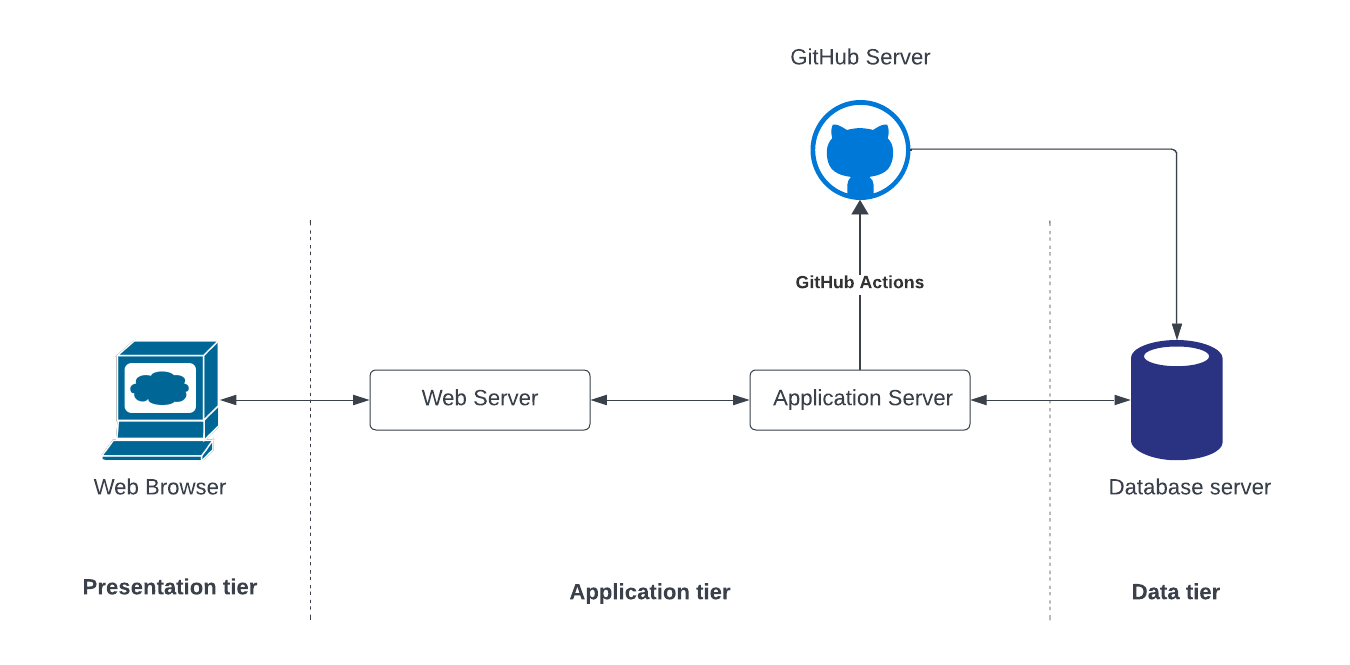
\includegraphics[width=\textwidth]{Graphics/Architecture/3-tier architecture.png}
    \caption{High level system architecture}
    \label{fig:3tierArchitecture}
\end{figure}

The external service integration most crucial to the CodeKataBattle's main functionality is the integration of GitHub. This is enabled through GitHub Actions which allows for the setting up of workflows that automate tasks based on events in specific GitHub repositories. This aspect falls under the system's Application Tier, which consists of the Webserver, the Application Server, and the communication with the Github Server. 

Regarding the internal set-up of the application tier, an event-driven architecture has been chosen, as this is greatly supported by GitHub Actions. The deployment of GitHub actions removes the necessity to build or integrate event brokers, publishers or subscribers, as this is handled by the action yaml-file (see fig. \ref{fig:EventFlow}). 

Every single Battle will simply consist of a standardised GitHub repository with standardised actions built in. The actions ensure that, upon a push to a forked repository, certain specified test files are run and the results are subsequently written to the database, if the push occurs within the battle time limit. 

The effective scaling of the testing modules in case of increased amount of submissions to a battle immediately before the deadline, has been identified as a potential bottleneck of the system. However, as GitHub Actions spins up an independent container for each event (e.g. a push) being handled, it harvests the strengths of a microservice architecture and averts this specific bottleneck.

The workload is split between three physical infrastructures; The submissions and testing occurs on GitHub’s infrastructure, The application is hosted on the application and web server, and the database containing the results are secluded on the database server (see fig. \ref{fig:physicalpartitions}). 
The Application Server "writes" to the GitHub server only to trigger the creation of a new battle repository upon educator input. In response GitHub actions provides the battle repository URL, which it writes to the database, from where the Application Server reads it. Thus the Application Server "writes" to the GitHub server and the Github server "writes" to the database (see fig. \ref{fig:3tierArchitecture}).

This physical dichotomy means that most of the workload is going to be placed on the container-based infrastructure of GitHub Actions, decreasing the requirements for the remaining infrastructure in order to remain scalable. The Web-server simply needs to support users reviewing their results and rankings of their battles, while all the scoring is handled in another system. While scoring of submissions are performed in relative parallel, potential bottlenecks can occur if many submissions are made at the same time, creating a long write-queue to the database, potentially increasing the time from a submission is made until the result is visible on the web app. Another potential bottleneck is simply that of many sign-ins and requests for battle results, for which we currently don't supply any mitigation strategy, as it is unclear how badly it will scale with user count.

\begin{figure}[H]
    \centering
    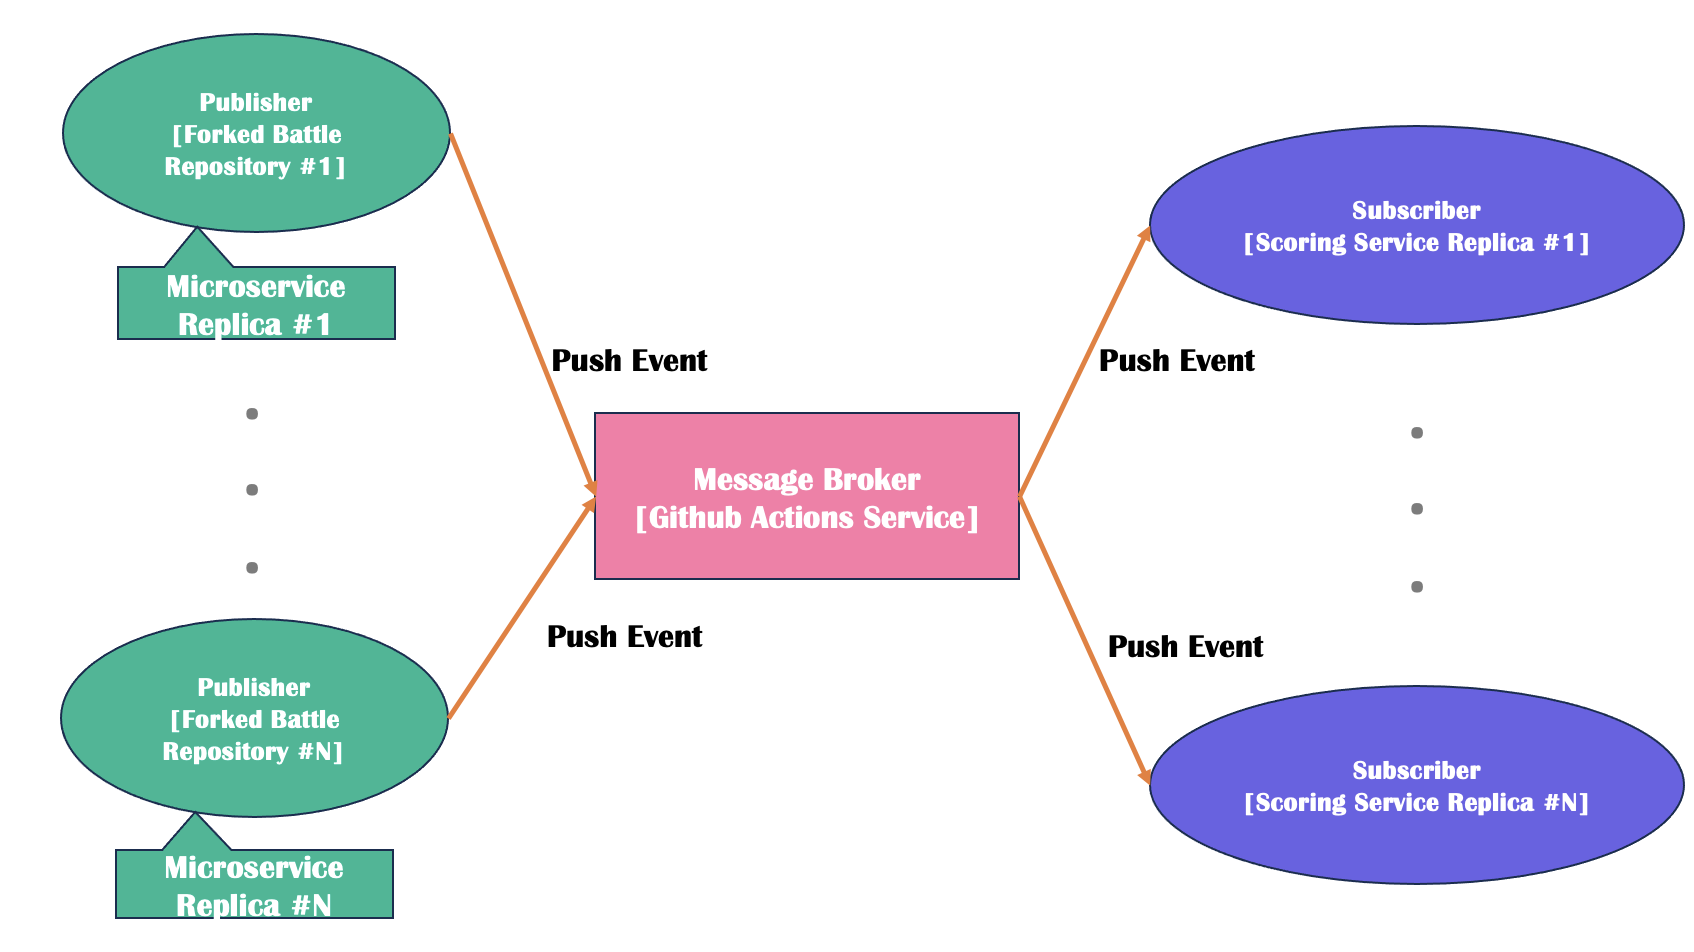
\includegraphics[width=\textwidth]{Graphics/Architecture/EventFlow.png}
    \caption{Event-driven architecture (Sub/Pub)}
    \label{fig:EventFlow}
\end{figure}


\begin{figure}[H]
    \centering
    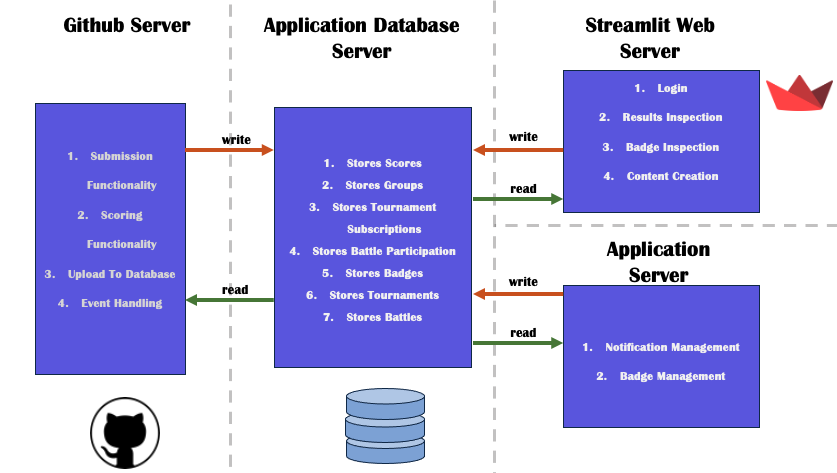
\includegraphics[width=\textwidth]{Graphics/Architecture/Physical Partitions.png}
    \caption{Physical Infrastructure Partitions}
    \label{fig:physicalpartitions}
\end{figure}


\subsection{Component view}
The components are organized into the following modules: \bigskip  \newline \textbf{User Interface Components}: \newline
 Responsible for rendering the web pages, handling user interactions, and making requests to the back-end. Individual components include:
\begin{itemize}
    \item \textbf{Front-end Service} \newline
    Represents the front-end of the application, handling user interactions, displaying information, and communicating with back-end services.
    \item \textbf{User Profile Service} \newline
    Manages user profiles, including the display of badges, tournament ranks, and overall performance visualisation
    \item \textbf{Educator Tools Service} \newline
    Provides tools and interfaces specifically for educators to create and manage tournaments, battles, and perform manual evaluations.
    \item \textbf{Authentication Service}
         \newline Responsible for user authentication and authorization.

    \item \textbf{Github Management Service}
        \newline Manages the creation and updates of relevant Github Repositories, as well as general automated communication with the Github API.
\end{itemize}
\textbf{Back-end Components}: \newline
 Responsible for processing user requests, performing application-specific functionalities and enabling the interactions between the presentation and data tier.
    \begin {itemize}
        
         %\item  \textbf{Tournament Management Service}
         %\newline Handles the creation, configuration, and management of tournaments, including setting up tournament details, deadlines, and badge criteria. It furthermore keeps track of tournament progress, participation, and tournament ranking.
         %\item  \textbf{Battle Management Service}
        %\newline Manages the creation, configuration, and deadlines of battles as well as the sign-up of participants. It triggers the creation of battle repositories through GitHub Actions, including the upload of the YAML file specific to the battle defining the submission tests customised by the educator upon battle creation. It keeps track of battle submission scores provided by the Scoring Service and updates battle rankings after each Git push.
        \item \textbf{Scoring Service}
         \newline Reads code submission test results from the database (written their by GitHub Actions) to calculate the teams battle score based on aspects such as number of tests passed, timeliness of submission and code quality levels.
        \item  \textbf{Badge Management Service}
        \newline Deals with the creation, assignment rules, and management of tournament badges. Assigns badges depending on the educator's defined rules at the end of each tournament.
        \item  \textbf{Notification Service}
        \newline Handles the notification system for informing users about new tournaments, battle updates, final battle results, and tournament badge achievements.
        \item  \textbf{Data Persistence Service (DBMS)}
        \newline Manages the storage and retrieval of data related to tournaments, battles, user profiles, scores, and badges.
         
    \end{itemize}
\textbf {GitHub Integration Components}: 

\begin{itemize}
    \item \textbf{GitHub Actions}
    \newline Used to set-up the event-driven automated testing of code submissions to forked battle repositories, upon each push. It stores test results to the system's database, where they are retrieved by the Scoring Service. GitHub Actions creates battle repositories, ultimately triggered by the Front-end Service.
\end{itemize}


\begin{figure}[H]
    \centering
    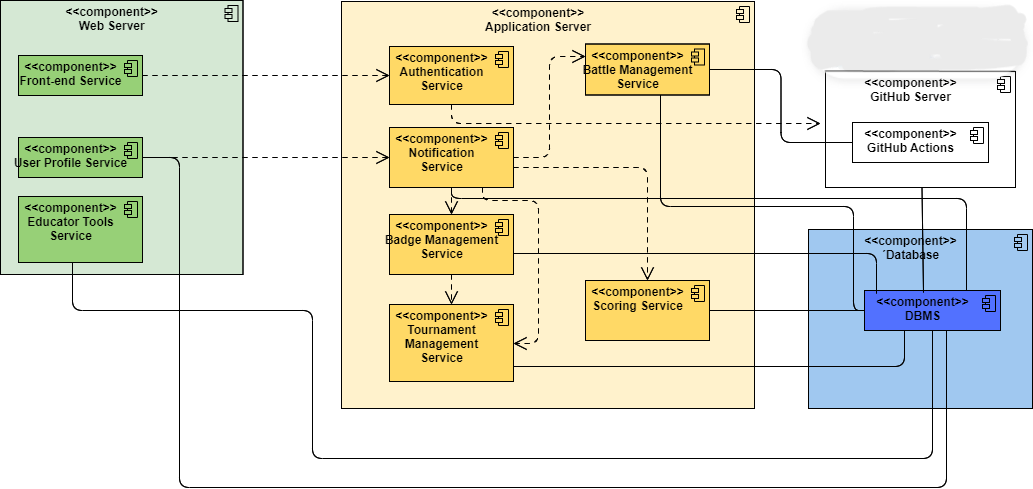
\includegraphics[width=\textwidth]{Graphics/Architecture/UML Component Diagram.png}
    \caption{Component Diagram}
    \label{fig:componentDiagram}
\end{figure}

\subsection{Deployment view}
The system will be deployed using a cloud-based infrastructure, ensuring scalability and availability. The deployment consists of:
\begin{itemize}
    \item \textbf {Web Server}: Hosts the web application accessible to users.
    \item \textbf {Application Server}: Hosts the backend modules responsible for business logic and data processing.
    \item \textbf {Database Server}: Stores user data, tournament and battle configurations, and results, as well as user data.
    \item \textbf {GitHub Actions}: Interacts with GitHub for repository hosting, version control, and automated battle code testing.
\end{itemize}
\subsection{Runtime views}
\newline
\subsubsection{Login Sequence}
\begin{figure}[H]
    \centering
    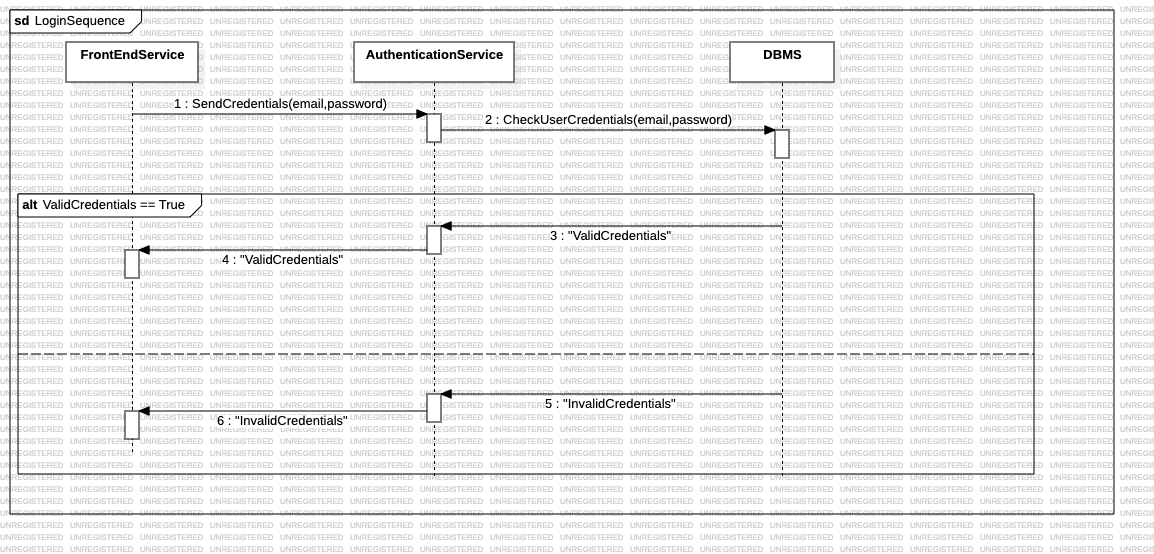
\includegraphics[width=\textwidth]{Graphics/Sequence Diagrams/LoginSequence.png}
    \caption{Login Sequence}
    \label{fig:login}
\end{figure}
The login-sequence in our case is quite simple, as the user simply inputs their credentials on the login page of the front-end. The credentials are then forwarded to the AuthenticationService which checks the validity of the credentials against the stored credentials in the DBMS. This functionality is the same, whether done as a Student User or an Educator User.

\subsubsection{Create Battle}

\begin{figure}[H]
    \centering
    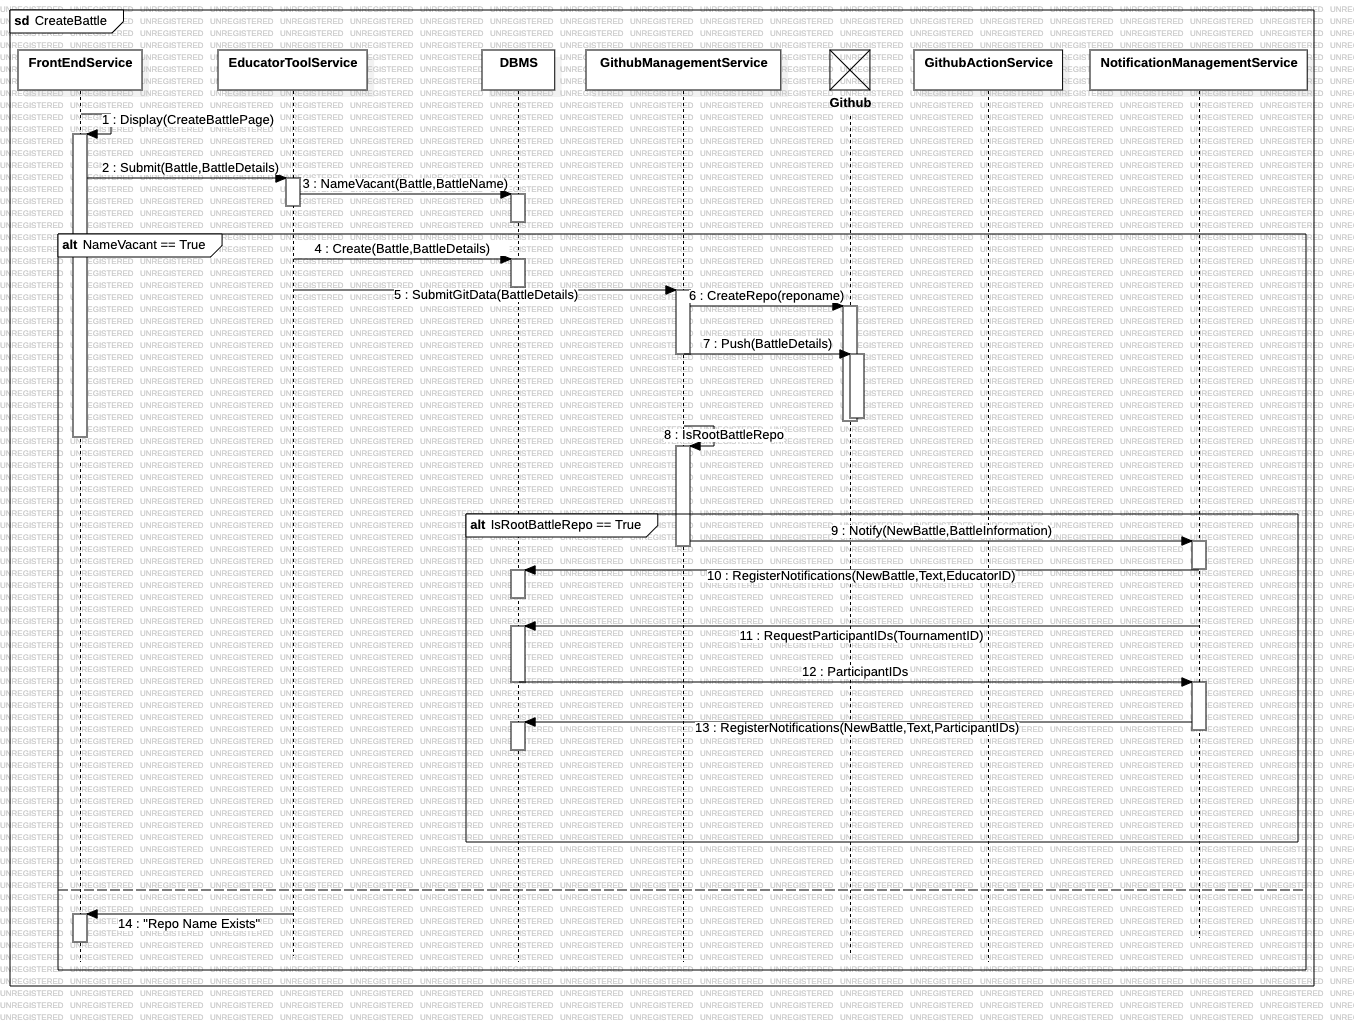
\includegraphics[width=\textwidth]{Graphics/Sequence Diagrams/CreateBattle.png}
    \caption{Create Battle}
    \label{fig:createbattle}
\end{figure}
When creating a battle in our chosen architecture, we can leverage the functionality and infrastructure of Github and Github Actions. When an Educator wishes to create a Battle, they do so through the front-end service, by simply filling in the battle details, such a name, sign-up deadline, submission deadline and description. Additionally, the Educator submits a series of test files that can be used to evaluate the submissions. When the Educator finalizes the battle creation, the front-end service first verifies that no other battle shares this name, as the name will be used in the creation of the battle's Github repository, which must be unique. If the name is unique, the Educator Tool Services can generate a repository name for the battle and officially create the Battle in the Database Management System. However, this only officially creates the Battle \textit{internally}, so a Github repository is then created from a Battle template-repository complete with Github Action YAML-files, relevant directories and so on through the Github Management Service. Subsequently, the relevant files and information from the Educator is pushed to the copied template. A check is performed to verify that this is, in fact, the root Battle repository, and not a forked submission repository. When this is verified, an action can activate the notification procedure using the Notification Management Service. The Notification Management Service first requests all userIDs of Students subscribed to the Tournament, to which this Battle belongs. Then Notifications of a new Battle is sent to all these users' email addresses.  


\subsubsection{Create Tournament}

\begin{figure}[H]
    \centering
    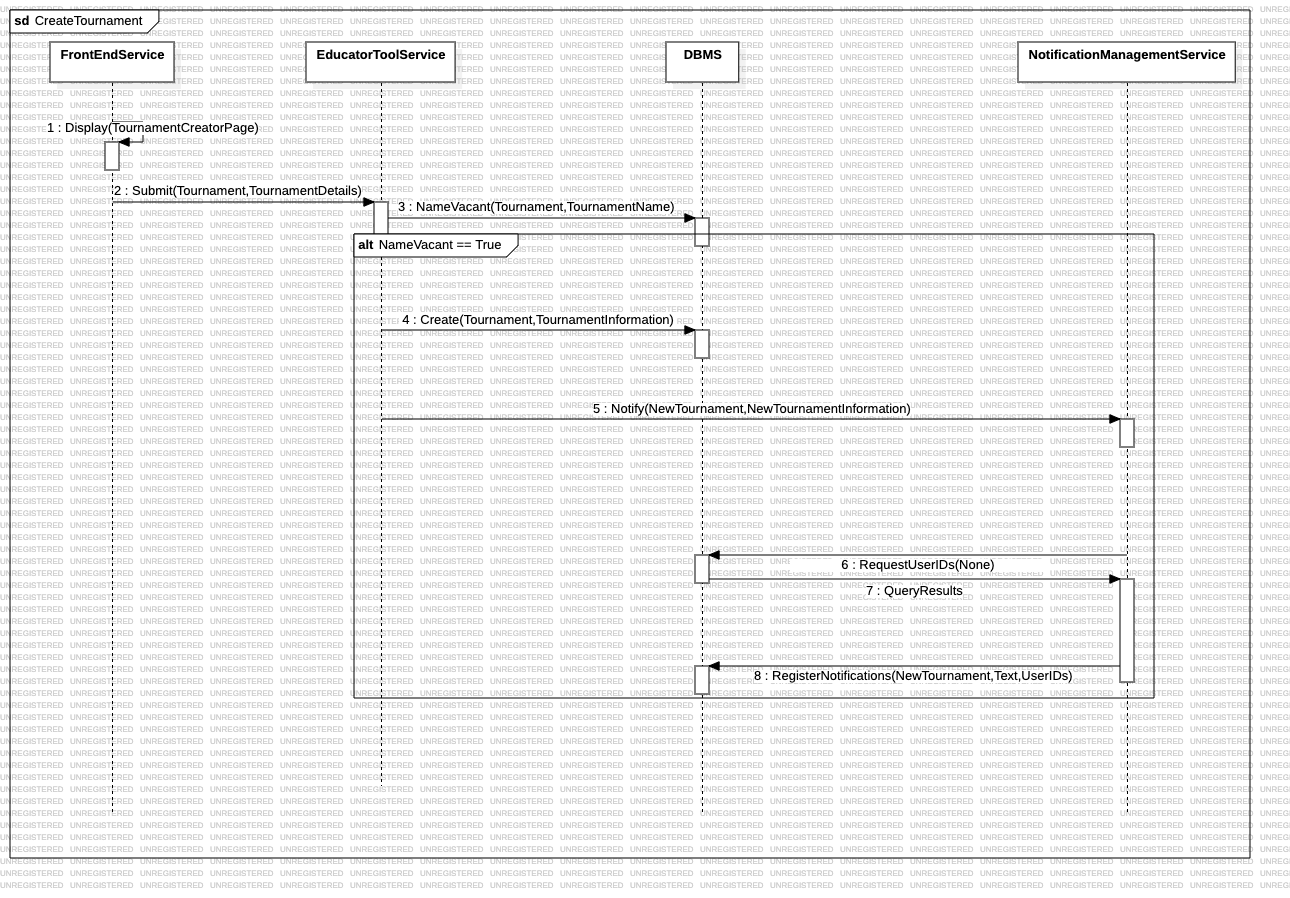
\includegraphics[width=\textwidth]{Graphics/Sequence Diagrams/CreateTournament.png}
    \caption{Create Tournament}
    \label{fig:createtournament}
\end{figure}
Creating a Tournament is much simpler than creating a Battle, as no repositories are involved yet. When an Educator creates a Tournament by filling out the CreateTournament-form through the Front-end service, the Tournament details are forwarded to the Educator Tool Service. This, in turn, checks whether the a Tournament of this name already exists. If not, the Educator Tool Service can officially create the Tournament in the DBMS. When the Front-end service refreshes, it will pick up the new Tournament from the DBMS.
Subsequently, a trigger with the relevant Tournament information is forwarded to the NotificationManagementService, which will notify all users on the platform that a new Tournament is available. 

\subsubsection{Create Badge}

\begin{figure}[H]
    \centering
    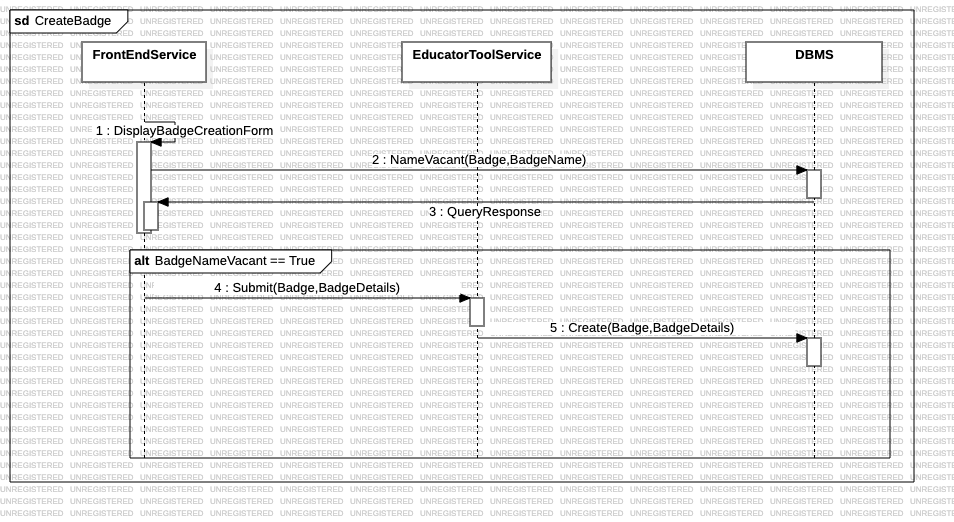
\includegraphics[width=\textwidth]{Graphics/Sequence Diagrams/CreateBadge.png}
    \caption{Create Badge}
    \label{fig:createbadge}
\end{figure}
When creating a Badge, the Educator uses the BadgeCreationForm from the FrontEndService. This form consists of a crude graphical user interface, that translates well into SQL queries. First, the Front-end Service ensures, that the badge name is unique to this tournament. If this is the case, the SQL-adjacent logic is forwarded to the Educator Tool service, and stored in the DBMS. 

\subsubsection{Receive Badge}
\begin{figure}[H]
    \centering
    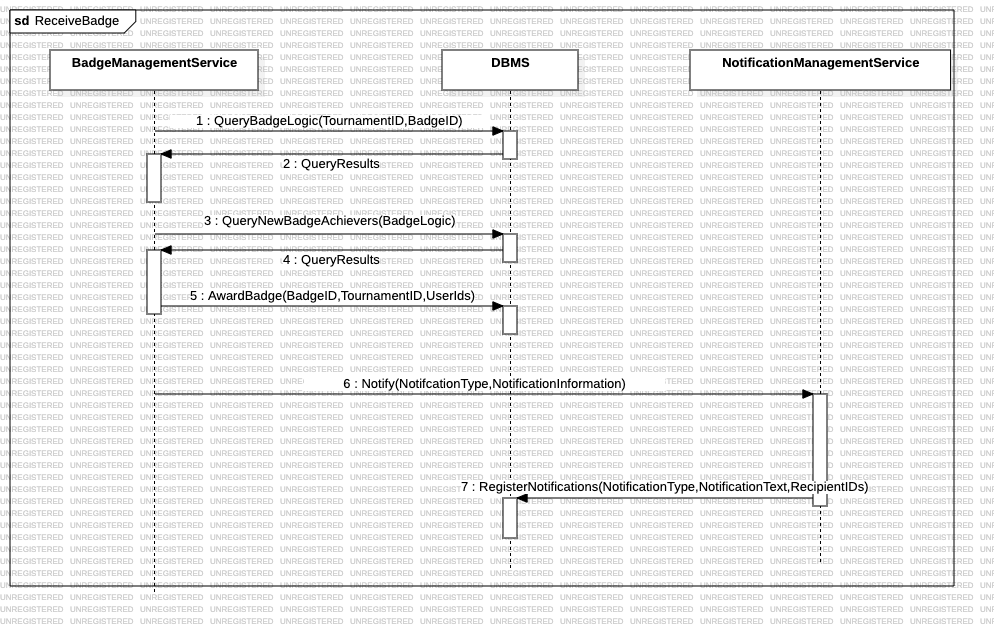
\includegraphics[width=\textwidth]{Graphics/Sequence Diagrams/ReceiveBadge.png}
    \caption{Receive Badge}
    \label{fig:receivebadge}
\end{figure}
There can potentially be quite a lot of variety in the events that can trigger a Badge. Therefore, the Badge management service simply performs a query each day, using the SQL-adjacent logic of the Badges, to retrieve all Students for all Tournaments that correspond to the queries, but have not been assigned the Badge. This solution, however, might scale poorly, as Tournaments may be active for years.

\subsubsection{Submit Solution}
\begin{figure}[H]
    \centering
    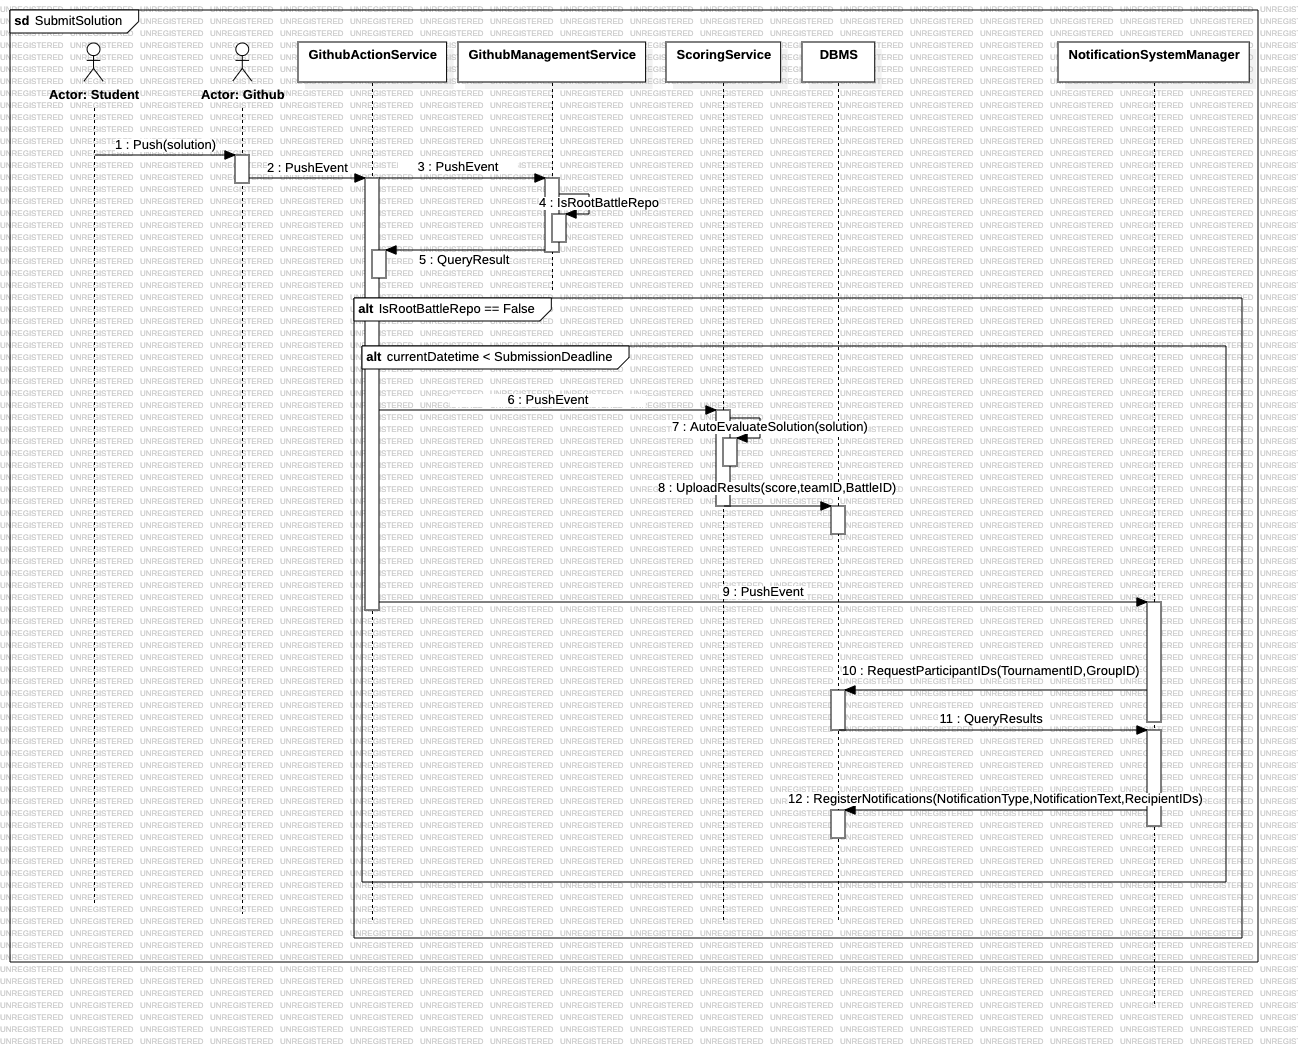
\includegraphics[width=\textwidth]{Graphics/Sequence Diagrams/SubmitSolution.png}
    \caption{Submit Solution}
    \label{fig:submitsolution}
\end{figure}
When making a Submission, we get to leverage the choice of architecture once more. When a Student performs a push to their forked Battle repository, before the deadline, it triggers the Github Action Service. The Github Action Service will follow the instructions in the Github Actions YAML-file and activate the Scoring service, automatically evaluating the Submission. The evaluation is then written to the DBMS. 
Subsequently, the YAML-file dictates that a Notification is sent to the users of the responsible group, by gathering the relevant userIDs from the DBMS.  

\subsubsection{Join Battle}
\begin{figure}[H]
    \centering
    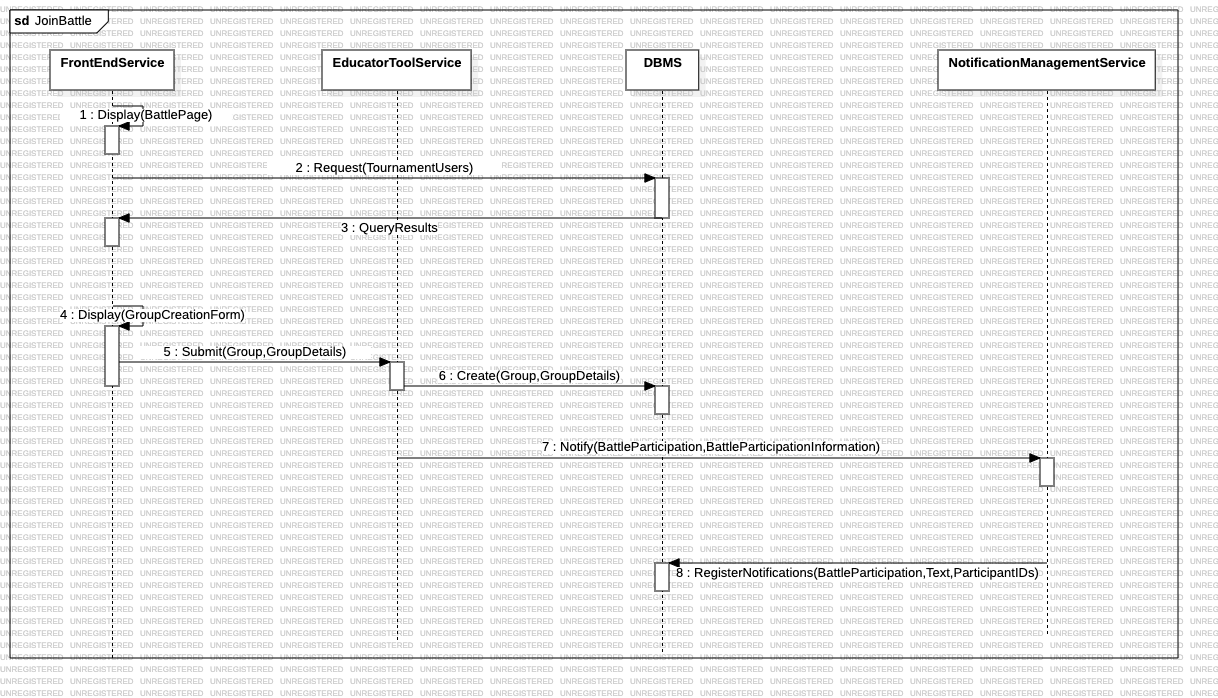
\includegraphics[width=\textwidth]{Graphics/Sequence Diagrams/JoinBattle.png}
    \caption{Join Battle}
    \label{fig:joinbattle}
\end{figure}
When joining a Battle from the Front End Service, a Student will be prompted with a drop down of the Students subscribed to the current Tournament without a group all retrieved from the DBMS. They can then select their preferred team mates, as long as they don't exceed the Educator determined threshold for group size.  The group is then written to the DBMS, through the Educator Tool Service, which manages all user-facing \textit{writes} to the DBMS, thus finalizing the group creation. The Notification Management Service is then triggered and notifies the users of their successful group formation, and Battle sign-up. 

\subsubsection{Manual Scoring}
\begin{figure}[H]
    \centering
    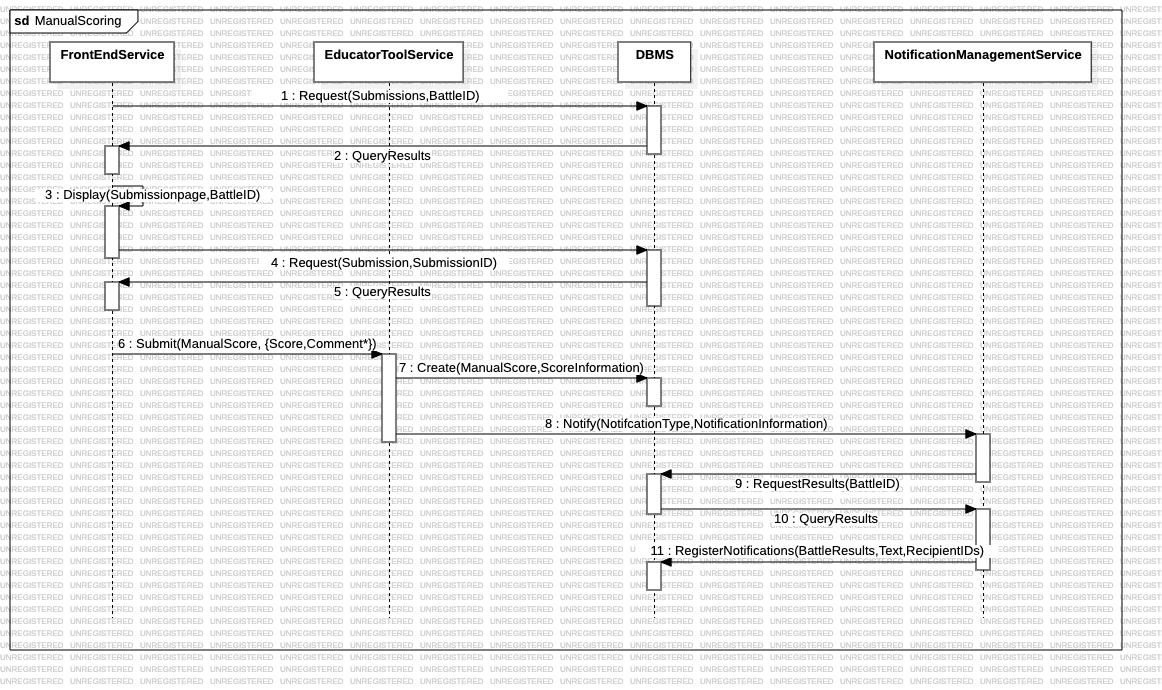
\includegraphics[width=\textwidth]{Graphics/Sequence Diagrams/ManualScoring.png}
    \caption{Manual Scoring}
    \label{fig:manualscoring}
\end{figure}
When a Battle has ended the Educator is able to assign a manual score, as well as a manual feedback to the Students. This is done throug the Front-end Service, which displays the Submissions from each Group which has received the maximum automated score. The Educator can then assign a score on the same range as the automated score, as well as a comment on the overall quality of the submission. This information is then written to the DBMS, and then notified to the responsible group through the Notification Management Service. 
The new scores will be available through the Front-end Service upon refresh. 


\subsubsection{Subscribe to Tournament}
\begin{figure}[H]
    \centering
    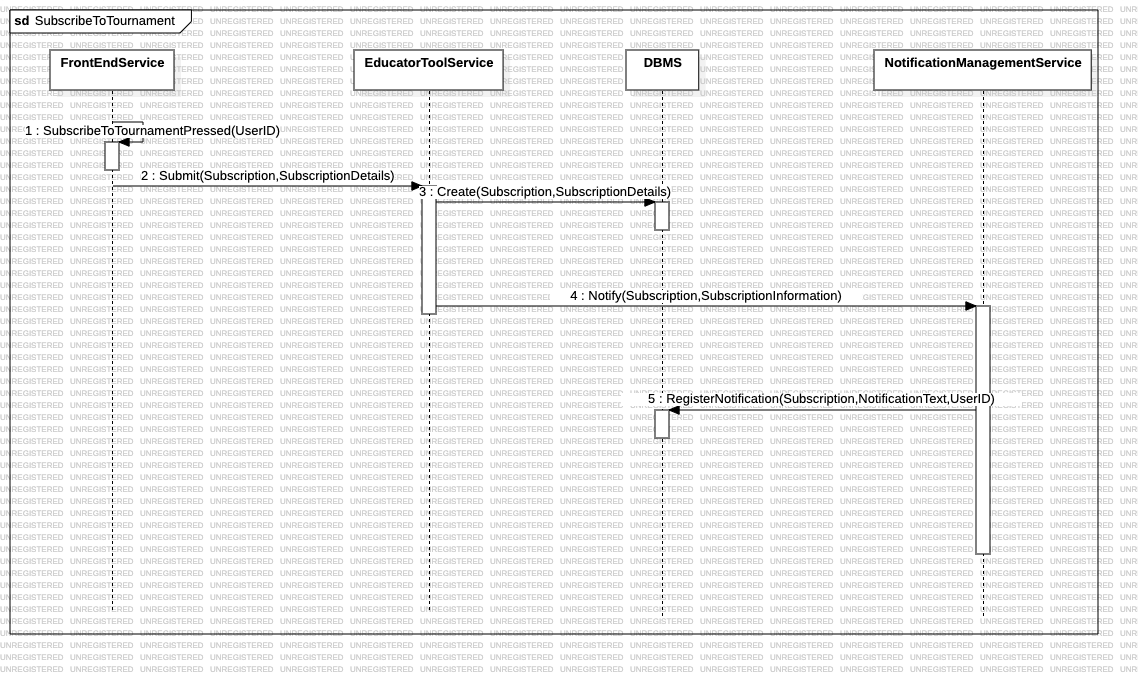
\includegraphics[width=\textwidth]{Graphics/Sequence Diagrams/SubscribeToTournament.png}
    \caption{Subscribe To Tournament}
    \label{fig:SubscribeToTournament}
\end{figure}
When a Student subscribes to a Tournament through the Front-end Service, their UserID is simply added to the DBMS, allowing the system to notify the Student of future Battles, as well as making them eligible to participate in these Battles. Immediately, the Front-end Service forwards the relevant information to the Notification Management Service, which in turn notifies the user of their successful subscription. 

\subsubsection{Announce Battle Results}
\begin{figure}[H]
    \centering
    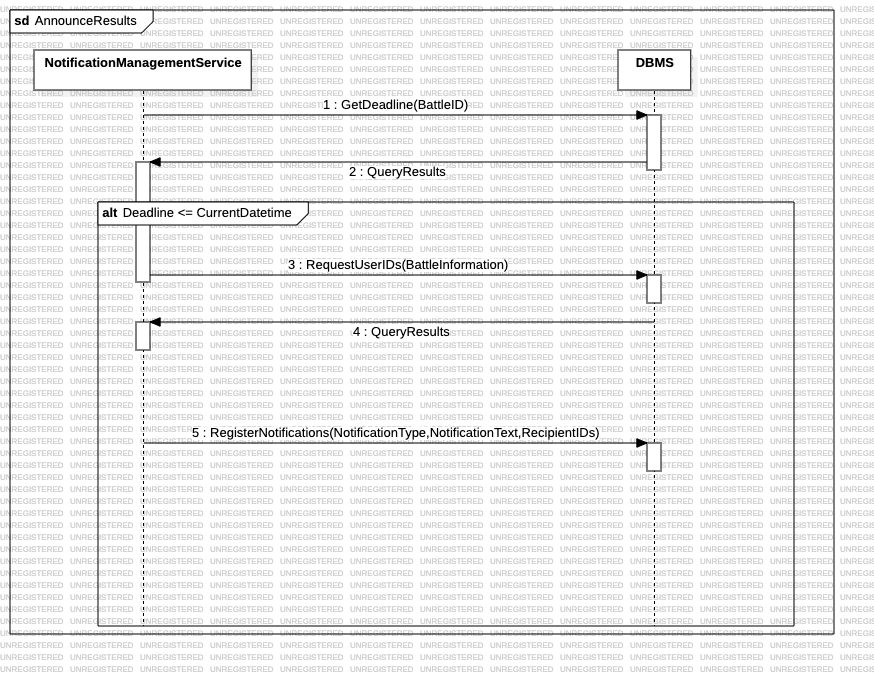
\includegraphics[width=\textwidth]{Graphics/Sequence Diagrams/AnnounceResults.png}
    \caption{Announce Battle Results}
    \label{fig:announceresults}
\end{figure}
Every day, the Notification Management Service, checks which Battles have ended since yesterday, by checking the DBMS. All participants of the Battle is then notified of their final ranking, which can also be found on the Battle page of the Front-end Service. 


\subsection{Component interfaces}
The following section aims at providing a complete list of all the methods each component interface provides to the other components.
(note: actual method names and parameters will be different based on the implementation details, we can change them later - consider these placeholders)
\bigskip \newline 
\textbf{User Interface Components}
\begin{itemize}
    \item \textbf{Front-end Service}
        \begin{itemize}
            \item Display(PageName,PageInformation)
            \item SendCredentials(email,password)
            \item Submit(Objecttype,Objectdetails)
            \item NameVacant(ObjectType,ObjectInformation)
            \item Request(data)
        \end{itemize}
    \item \textbf{User Profile Service}
        \begin{itemize}
            \item displayUserProfile(userID)
            \item updateUserProfile(userID, newProfileData)
        \end{itemize}
    \item \textbf{Educator Tools Service}
        \begin{itemize}
            \item Create(Objecttype,Objectdetails)
            \item NameVacant(ObjectType,ObjectInformation)
            \item Notify(NotifcationType,NotificationInformation)
            \item SubmitGitData(BattleDetails)
        \end{itemize}
\end{itemize}

\textbf{Back-end modules}

\begin{itemize}
    \item \textbf{Authentication Service}
        \begin{itemize}
            \item checkUserCredentials(userName, userPassword)
        \end{itemize}
    \item \textbf{Github Management Service}
        \begin{itemize}
            \item updateParticipantList(userID, teamID)
            \item IsRootBattleRepo()
            \item CreateRepo(RepoName)
            \item Push(PushDetails)
            \item Notify(NotifcationType,NotificationInformation)
        \end{itemize}
    \item \textbf{Scoring Service}
        \begin{itemize}
            \item AutoEvaluateSolution(solution)
            \item UploadResults(score,teamID,BattleID)
        \end{itemize}
    \item \textbf{Badge Management Service}
        \begin{itemize}
            \item AwardBadge(TournamentID,BadgeID,UserIDs)
            \item QueryBadgeLogic(BadgeID)
            \item QueryBadgeAchievers(BadgeLogic)
            \item Notify(NotifcationType,NotificationInformation)
        \end{itemize}
    \item \textbf{Notification Service}
        \begin{itemize}
            \item RegisterNotification(NotificationType,NotificationText,RecipientIDs)
            \item SendNotifications(NotificationType,NotificationText,RecipientIDs)
            \item RequestUserIDs(ObjectInformation)
            \item RequestDeadline(BattleID)
            \item RequestResults(BattleID)
        \end{itemize}
\end{itemize}


\subsection{Selected architectural styles and patterns}  

\subsubsection{three-tier architecture}
The system adopts a three-tier architecture differentiating between: 
\begin{itemize}
    \item \textbf{Presentation (User interface tier)}
    \begin{itemize}
        \item \textbf{Responsibility}: The presentation tier is the topmost layer and is responsible for presenting the application's user interface and handling user interaction.
        \item \textbf{Components}: This tier includes components such as user interfaces, graphical elements, and client-side logic.
        \item \textbf{Interaction}: It interacts directly with end-users, collecting user input and displaying results.
    \end{itemize}
    \item \textbf{Application logic (Business logic tier/middle tier})
    \begin{itemize}
        \item \textbf{Responsibility}: The application tier contains the business logic or application logic that processes user requests, performs application-specific functionality, and manages the communication between the presentation and data tiers.
        \item \textbf{Components}: This tier includes server-side logic, application servers, and by extension the external GitHub Server for processing business rules and workflows.
        \item \textbf{Interaction}: It communicates with both the presentation tier, the data tier, and the external service of GitHub Actions, orchestrating the flow of data and application functionality. 
    \end{itemize}
\item \textbf{Data management (Database tier)}
    \begin{itemize}
        \item \textbf{Responsibility}: The data tier is responsible for managing and storing data. It stores and retrieves data based on requests from the application tier.
        \item \textbf{Components}: This tier includes databases, data storage systems, and any components related to data storage and retrieval.
         \item \textbf{Interaction}: It interacts with the application tier to store and retrieve data as needed.
    \end{itemize}
\end{itemize}

\subsubsection{Event-Driven Architecture}
To manage the general flow of the system an event-driven architecture is adopted. In an event-driven architecture three subsystems are considered:
\begin{itemize}
    \item \textbf{Publisher:} The individually forked Battle repositories act as the Publisher of events in this system. This means that the amount of Publishers for each Battle is equal to the number of participating teams. The forked repositories have the ability to trigger one certain event; \textbf{push}.  
    
    \item \textbf{Event Broker:} The Event Broker in our system is embodied by the Github Actions Service (GAS). When a push event occurs, GAS forwards the event to the "subscribers". 
    
    \item \textbf{Subscriber:} The Subscriber in our system is the concrete GitHub Action Replica, that runs certain code whenever an event occurs. In our case, the subscriber will check if the submission is made within the time limit, making it eligible for scoring, and if so run the scoring service. 
\end{itemize}

 
\subsection{Other design decisions}
\begin{itemize}
    \item \textbf {Web Application Development Platform}: The CodeKataBattles web application will be developed using the Streamlit platform. Streamlit provides a comprehensive set of tools, libraries, and frameworks that streamline web development, ensuring efficiency.
    \item \textbf{Scalability}: %The system is designed to scale horizontally by adding more servers to the infrastructure to handle increased user load during peak times.
    The system is designed to scale vertically by upgrading the machine the system runs on. Scaling horizontally would require implementing a load balancer, which is infeasible for this minimum viable product, but the best approach when further scaling the platform. 
    \item \textbf{Security}: HTTPS is enforced for secure communication, and user authentication is handled using OAuth through GitHub credentials. We have decided to funnal all write functionality from the UI through a single service in the system (Educator Tool Service), in order to decrease the sources of potential SQL-injections. 
    \item \textbf{Caching}: Caching mechanisms are implemented to optimize data retrieval and enhance system performance.
\end{itemize}

 \subsubsection{Availability}
As described in the RASD document, the requirements of the availability of our system are not tremendous. This is in part due to the relatively low importance of this type of software, as compared to software handling critical infrastructure, sensitive data or life supporting systems. However, due to the chosen design of the system, most of the information related to ongoing battles, such as the Battle-tests, Submissions, Version control and so on, is all stored on Github's infrastructure. This means that, in the case of a breakdown, all Students in on going Battles, can continue their work, relatively unaffected, and simply receive their evaluations when the service returns. All submissions are timestamped in Github's systems, so all submissions made before the deadline will still be regarded, even if the deadline has been passed during an outage. 

 \subsubsection{Data Storage}
This architectural design aims to provide a scalable, secure, and maintainable platform for CodeKataBattles, aligning with the specified requirements.
\section{User Interface Design}
For all visualization of the intended User Interface, we refer to the RASD document. 
\clearpage
\newpage
\section{Specific Requirements}
\label{sec:reqs}
%include more details on all aspects of section 2 if they are useful for the development team

\subsection{External Interface Requirements}
\subsubsection{User Interfaces}
This section presents the user interfaces for the CodeKataBattles platform. The first section is dedicated to the user interfaces encountered by the student, and the second section to those encountered by the educator. While similar on many accounts as both students and educators need the ability to monitor and receive notifications about relevant tournaments and battles. However, students' interactions with battles and tournaments are limited to monitoring and subscribing, while educators can create new battles and tournaments. While the service needs to be accessed by a heterogeneous set of users, because a lot of the intricacies of the difference in use-cases are handled by GitHub, a lot of the functionalities available to students and educators are very closely related. 

\newpage
\clearpage
\subsection{Students}

\begin{figure}[Htbp!]
    \centering
    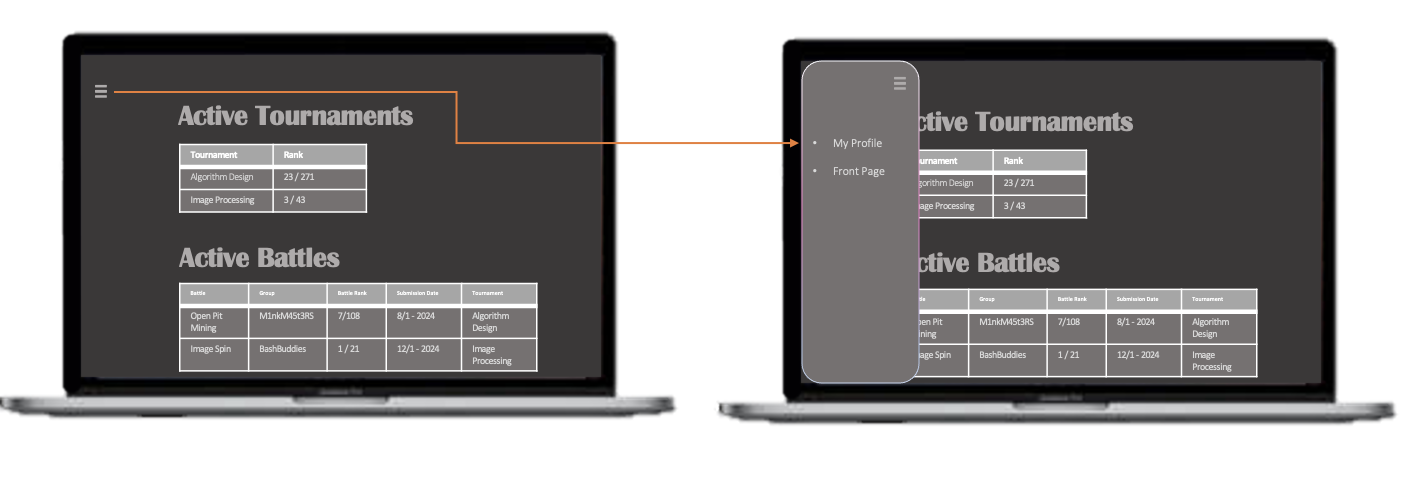
\includegraphics[width=\textwidth]{Graphics/SIDE BAR.png}
    \caption{User Interface: Front Page \& Sidebar}
    \label{fig:Sidebar}
\end{figure}

\begin{figure}[Htbp!]
    \centering
    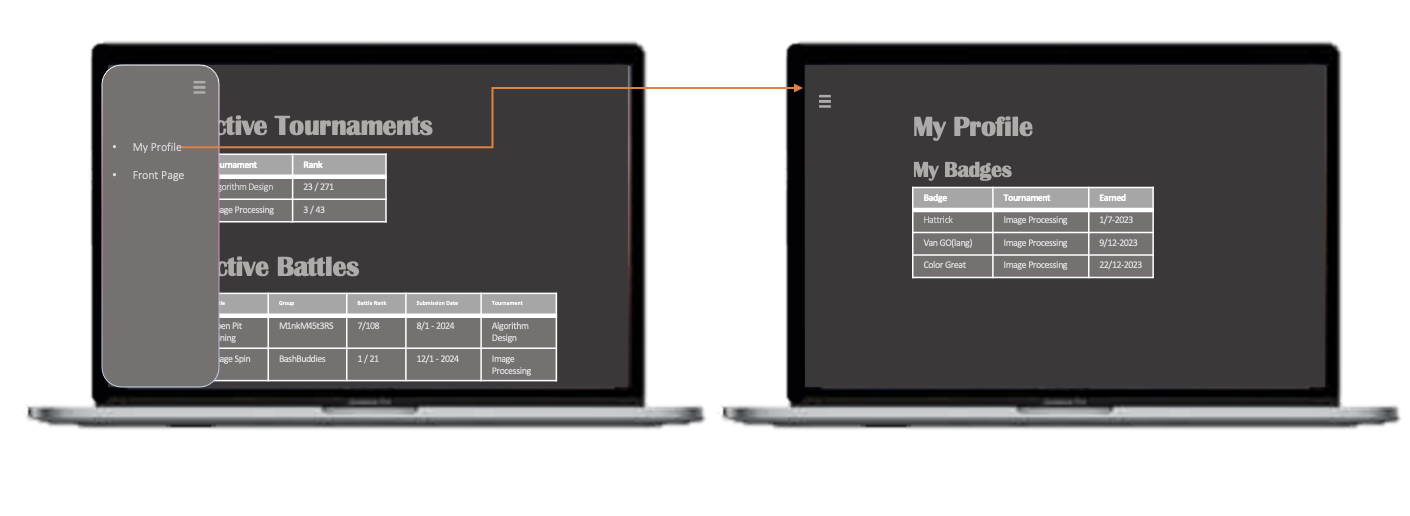
\includegraphics[width=\textwidth]{Graphics/MY PROFILE.png}
    \caption{User Interface: Profile}
    \label{fig:profile}
\end{figure}

\begin{figure}[Htbp!]
    \centering
    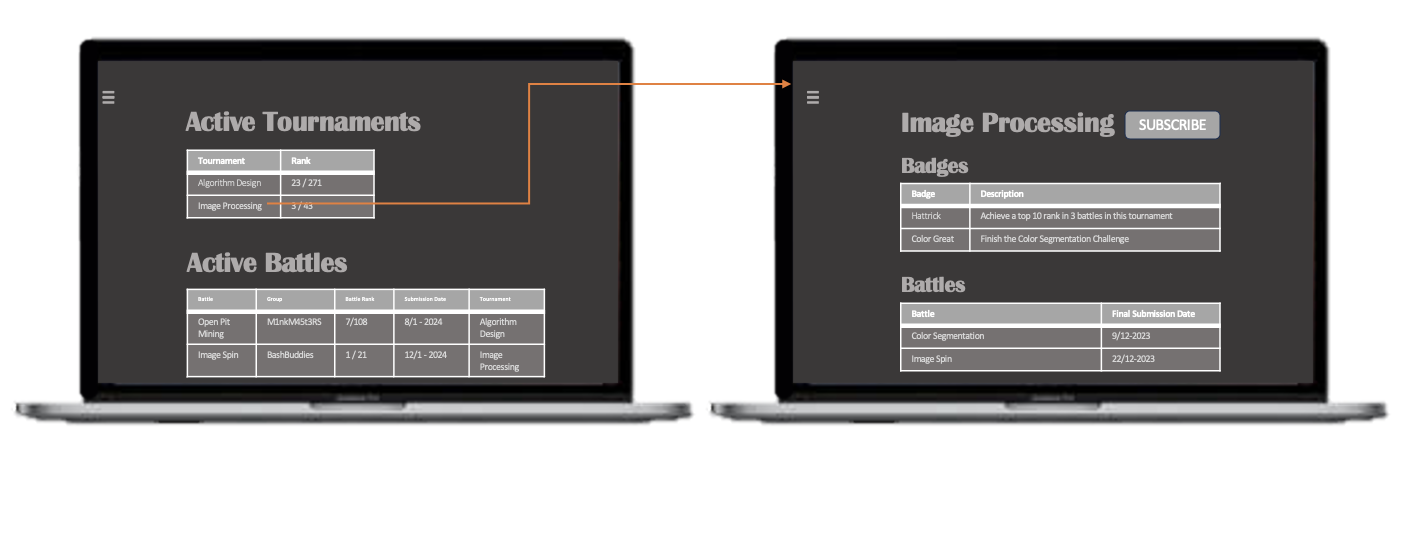
\includegraphics[width=\textwidth]{Graphics/TOURNAMENTS.png}
    \caption{User Interface: Tournament Page}
    \label{fig:tournaments}
\end{figure}


\begin{figure}[Htbp!]
    \centering
    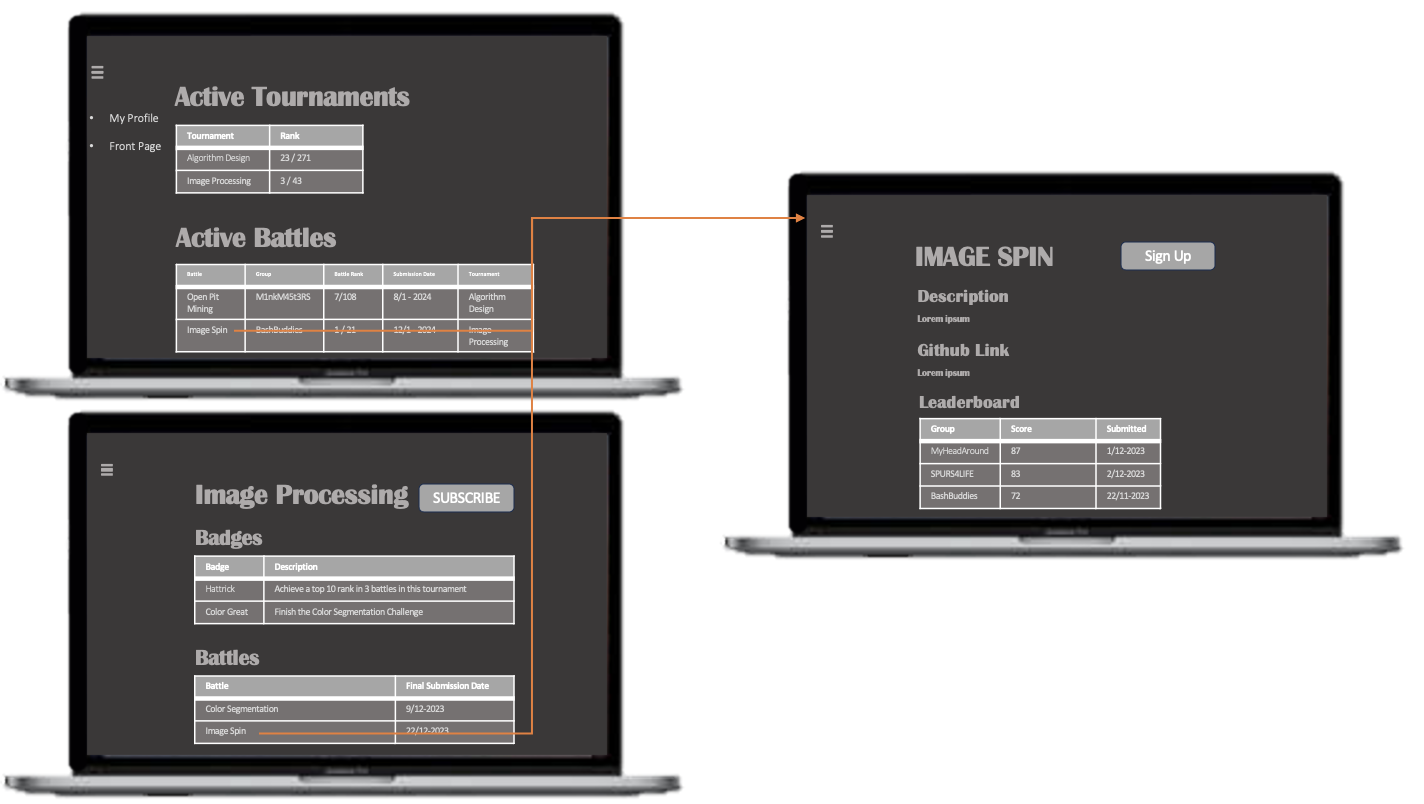
\includegraphics[width=\textwidth]{Graphics/BATTLE.png}
    \caption{User Interface: Battle Page}
    \label{fig:battle}
\end{figure}


\begin{figure}[Htbp!]
    \centering
    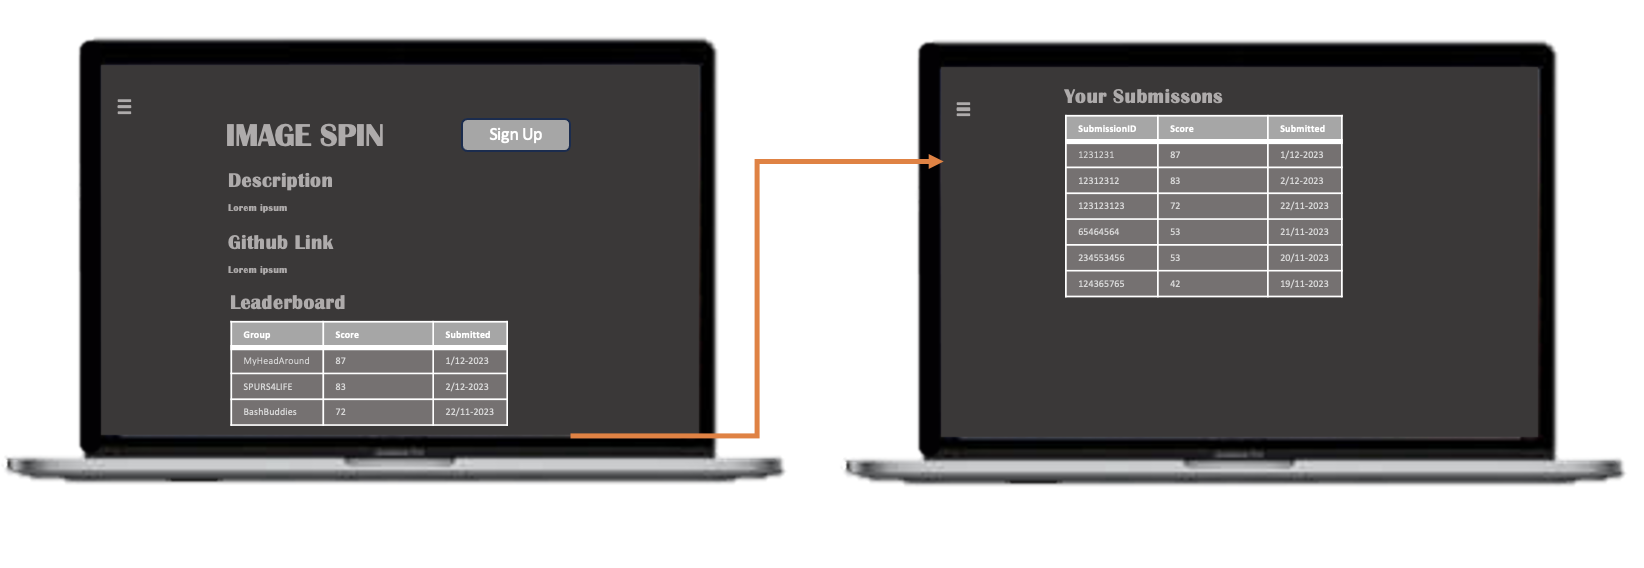
\includegraphics[width=\textwidth]{Graphics/SUBMISSION LOG.png}
    \caption{User Interface: Battle Page (Submission Log)}
    \label{fig:submissionlog}
\end{figure}

\subsection{Educators}

\begin{figure}[Htbp!]
    \centering
    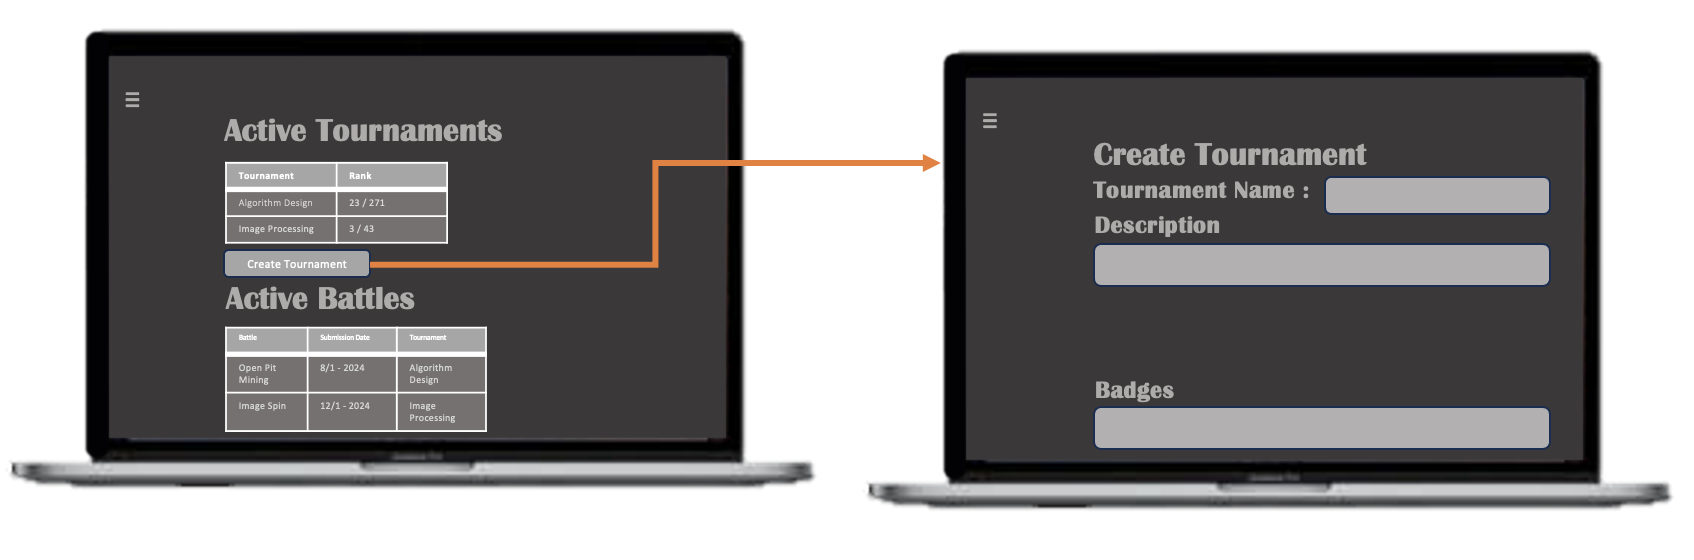
\includegraphics[width=\textwidth]{Graphics/CREATE TOURNAMENT.png}
    \caption{User Interface: Create Tournament Page}
    \label{fig:createTournament}
\end{figure}


\begin{figure}[Htbp!]
    \centering
    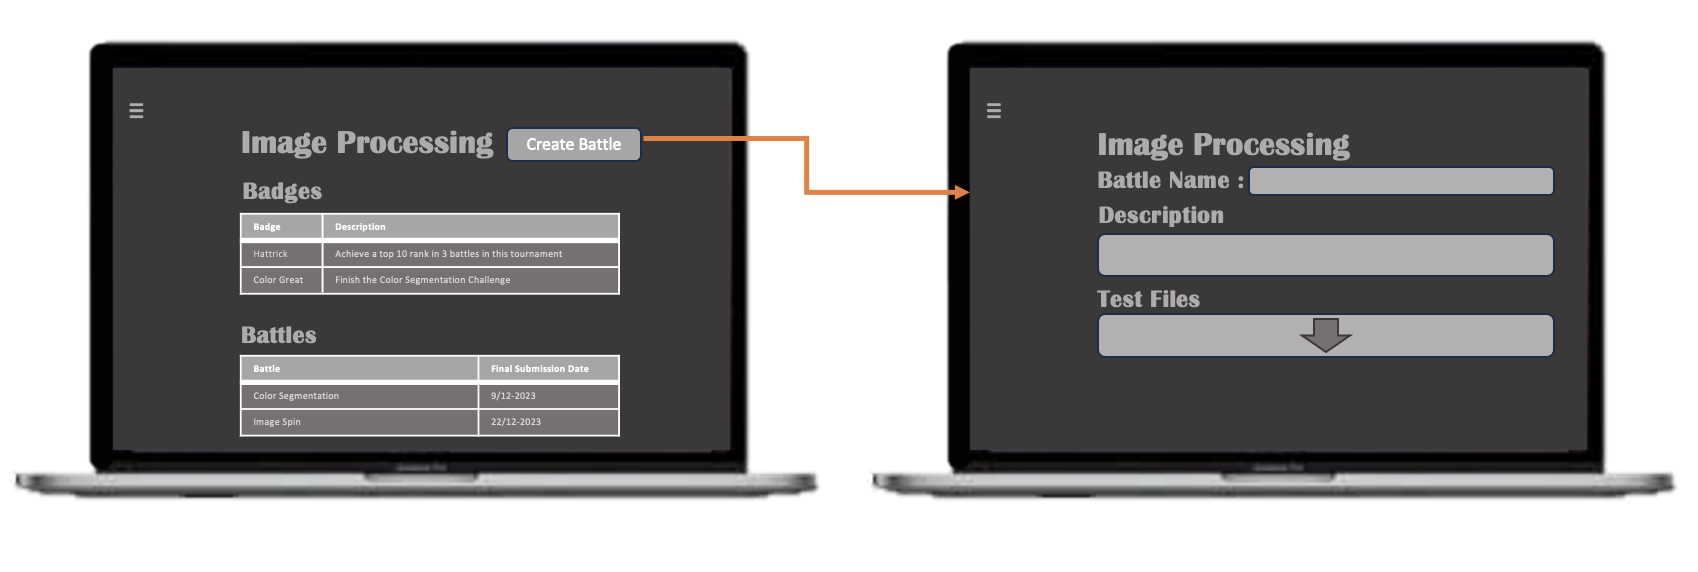
\includegraphics[width=\textwidth]{Graphics/CREATE BATTLE.png}
    \caption{User Interface: Create Battle Page}
    \label{fig:createBattle}
\end{figure}


\subsubsection{Hardware Interfaces}
All users, both Students and Educators can access the platform through a web browser. Therefore, all users need access to a device with an internet connection and browser installed. While note strictly required, a text editor is also recommended. 

\subsubsection{Software Interfaces}
The system utilizes one primary external service, namely Github. A Github action is set up, such that any pushes to a forked repository from a given battle is automatically pulled by the system. Then a predefined test script evaluates the implementation on a variety of tests.  

\subsection{Functional Requirements}
\label{sec:functional_requirements}

The CodeKataBattle system is designed to facilitate and manage competitive coding exercises, known as code katas. The system shall support the following functional requirements to ensure a comprehensive and engaging learning experience for students:

\begin{enumerate}
    \item \textbf{[R1]} The system shall allow users to sign up using their GitHub credentials (i.e. their email and GitHub Username).
    \item \textbf{[R2]} The system shall send a verification email to confirm a user's account upon sign-up.
    \item \textbf{[R3]} Educators shall be able to create tournaments with a specified title.
    \item \textbf{[R4]} Educators shall be able to set registration deadlines for tournaments.
    \item \textbf{[R5]} Educators shall be able to define tournament badge criteria.
    \item \textbf{[R6]} The system shall notify users of new tournaments.
    \item \textbf{[R7]} Users shall be able to subscribe to tournaments by a given deadline.
    \item \textbf{[R8]} Educators shall be able to create battles within tournaments.
    \item \textbf{[R9]} Educators shall be able to upload technical documents for battles.
    \item \textbf{[R10]} Educators shall be able to set the minimum and maximum number of students per group for battles.
    \item \textbf{[R11]} Educators shall be able to set a registration deadline for battles.
    \item \textbf{[R12]} Educators shall be able to set a final submission deadline for battles.
    \item \textbf{[R13]} Educators shall be able to configure scoring methodologies for battles.
    \item \textbf{[R14]} Students shall be able to form teams to join battles.
    \item \textbf{[R15]} The system shall provide a GitHub repository link for the code kata to registered teams after the registration deadline.
    \item \textbf{[R16]} The system shall automatically score submissions based on the results of test cases.
    \item \textbf{[R17]} The system shall evaluate the timeliness of submissions.
    \item \textbf{[R18]} The system shall assess the quality level of source code through static analysis.
    \item \textbf{[R19]} Educators shall have the option to manually score submissions.
    \item \textbf{[R20]} The system shall update battle scores in real-time upon new commits on GitHub.
    \item \textbf{[R21]} The system shall notify participants of final battle ranks after the consolidation phase.
    \item \textbf{[R22]} The system shall update personal tournament scores with the sum of battle scores.
    \item \textbf{[R23]} The system shall maintain a visible tournament rank for each student.
    \item \textbf{[R24]} Educators shall be able to define gamification badges with specific rules.
    \item \textbf{[R25]} The system shall display badges on student profiles.
    \item \textbf{[R26]} Educators shall be able to close tournaments and trigger final rank notifications.
    \item \textbf{[R27]} The system shall enable boolean expressions to define rules of badges and achievements.
    \item \textbf{[R28]} Students shall be able to visualize their performance.
    \item \textbf{[R29]} Students shall be able to visualize their tournament information.
    \item \textbf{[R30]} Students shall be able to track their battle involvement.
    \item \textbf{[R31]} Students shall be able to see detailed logs of their attempt outcomes.
\end{enumerate}

Definition of use case diagrams, use cases and associated sequence/activity diagrams, and mapping on requirements
 
\subsection{Performance Requirements}
\label{sec:performance_requirements}
The CodeKataBattles platform, recognizing the unique nature of code kata activities, has tailored performance requirements, especially concerning system downtime. Since a substantial part of the participation occurs in personal text editors or IDEs, the platform can accommodate longer downtimes without significantly impacting user productivity. An accepted downtime of up to half an hour is considered reasonable, allowing users to continue their work offline during such periods.

To minimize disruption, scheduled maintenance is planned during off-peak hours, and users are notified in advance through various channels. In case of unexpected downtimes, prompt communication is ensured, providing users with information and an estimated resolution time. Despite this tolerance for downtime, ensuring data integrity remains paramount. The platform is equipped with robust backup mechanisms to safeguard user data and maintain accessibility after downtimes.

These performance requirements reflect a balance between user experience and the practicalities of system maintenance for CodeKataBattles, catering to the platform's specific workflow.




\subsection{Design Constraints}

\subsubsection{Standards compliance}
Regarding data privacy, the CKB platform adheres to the General Data Protection Regulation (GDPR), which governs data protection and privacy for individuals within the European Union (EU) and the European Economic Area (EEA). Additionally, the system must comply with international standards for using and representing dates and times.

\subsubsection{Hardware limitations}
Here we report relevant hardware requirements. The only real hardware requirement is a machine with an Internet connection (2G/3G/4G/Wi-Fi) and a modern web browser

\subsection{Software System Attributes}
\subsubsection{Reliability}
As mentioned in section \ref{sec:performance_requirements} this service does not warrant complex infrastructure to aggressively reduce downtime, due to the amount of work being done in text editors or IDEs not directly connected to the platform. This is also the case for data, as all code is stored in Github repositories, however, all data related to the gamification aspect of the platform is stored only in the system. 

\subsubsection{Security}
As for any system handling personal information, such as CodeKataBattles does with information regarding educators and students, security is vital. 
To ensure compliance with security standards, encryption of passwords within the database must be applied. The same encryption need is present for data in transmission over the internet, to avoid interception-tactics. User's access to data must be a constraint to information deemed relevant for them through the use of role-based access control. 

\subsubsection{Availability}
CodeKataBattles is not a critical service, so the availability role is mainly to create a good user experience. Furthermore as mentioned in \ref{sec:performance_requirements} user productivity can exist in downtime. Therefore the system should aim to provide at least 99\% availability, meaning that the average time between occurrences of a failure and
service recovery (MTTR) must be less or equal to 3,65 days per year. 

\subsubsection{Maintainability}
The system is required to ensure a high level of maintainability. This entails the utilization of appropriate design patterns and adherence to recognized coding standards. The code must be well-documented, and practices such as hard-coding are strictly avoided. Moreover, the system should include a comprehensive testing routine, which is expected to cover a minimum of 75\% of the entire codebase, with the exception of interface code.

\subsubsection{Portability}
The web application should be compatible with all operating systems that support a web browser, including Windows, macOS, Linux, and others.

\begin{table}[h!]
\centering
\begin{tabular}{|p{0.2\textwidth}|p{0.7\textwidth}|}
\hline
\textbf{Name} & Login User \\
\hline
\textbf{Actors} & Student \& educator \\
\hline
\textbf{Entry Condition} & The student/educator has opened the CodeKata web application \\
\hline
\textbf{Event flow} & 
\begin{minipage}[t]{0.7\textwidth}
1 - The user inserts his username and password in the form \\
2 - The user clicks on the “Login” button \\
3 - The system checks the credentials \\
4 - The application shows the proper dashboard
\end{minipage} \\
\hline
\textbf{Exit condition} & The user has access to the services for the right interface provided by the CodeKata web application \\
\hline
\textbf{Exception} & 
\begin{minipage}[t]{0.7\textwidth}
3 - The data inserted are not valid. The system returns to the entry condition.
\end{minipage} \\
\hline
\end{tabular}
\caption{Use Case Specification}
\end{table}


\begin{table}[h!]
\centering
\begin{tabular}{|p{0.2\textwidth}|p{0.7\textwidth}|}
\hline
\textbf{Name} & Join tournament \\
\hline
\textbf{Actors} & Student \\
\hline
\textbf{Entry Condition} & 
\begin{minipage}[t]{0.7\textwidth}
1 - The student is logged into the CodeKata platform \\
2 - The student is on the home page of the CodeKata web application \\
3 - The registration deadline has not yet passed
\end{minipage} \\
\hline
\textbf{Event flow} & 
\begin{minipage}[t]{0.7\textwidth}
1 - The student selects one of the available tournaments on the homepage \\
2 - The student clicks on the “Join” button \\
3 - The system adds the specific user to the participant list for the given tournament \\
4 - The tournament is added to the overview of tournaments the student is currently participating in
\end{minipage} \\
\hline
\textbf{Exit condition} & 
The student now has access to the battles within the tournament and is returned to the tournament home page \\
\hline
\textbf{Exception} & \\
\hline
\end{tabular}
\caption{Use Case Specification}
\end{table}


\begin{table}[h!]
\centering
\begin{tabular}{|p{0.2\textwidth}|p{0.7\textwidth}|}
\hline
\textbf{Name} & Join battle \\
\hline
\textbf{Actors} & Student \\
\hline
\textbf{Entry Condition} & 
\begin{minipage}[t]{0.7\textwidth}
1 - The student is logged in \\
2 - The student is subscribed to the tournament, to which the battle belongs \\
3 - The battle is open for registration \\
4 - The student resides on the battles page
\end{minipage} \\
\hline
\textbf{Event flow} & 
\begin{minipage}[t]{0.7\textwidth}
1 - The student clicks on the “Join” button \\
2 - The student is prompted to specify participant(/s) by username in its group \\
3 - The student enters the name of the group \\
4 - The system adds the specific user/team to the participant list for the given battle \\
5 - The battle is added to the overview of battles the student is currently participating in
\end{minipage} \\
\hline
\textbf{Exit condition} & 
The student will now receive notifications relevant to the given battle and is returned to the battle's home page \\
\hline
\end{tabular}
\caption{Use Case Specification}
\end{table}




% Skal lige kigges over de her tables 
\begin{table}[h!]
\centering
\begin{tabular}{|l|l|}
\hline
\textbf{Name} & Create Battle \\
\hline
\textbf{Actors} & Educator \\
\hline
\textbf{Entry Condition} & 
\begin{tabular}[c]{@{}l@{}}
1 - The educator is logged into the CodeKata platform. \\
2 - The educator has the details of a specific tournament displayed. \\
\end{tabular} \\
\hline
\textbf{Event flow} & 
\begin{tabular}[c]{@{}l@{}}
1 - The educator clicks the “Create Battle” button. \\
2 - The educator uploads a brief textual description of the battle. \\
3 - The educator uploads a software project with build automation scripts. \\
4 - The educator sets the registration and submission deadlines. \\
5 - The educator selects the scoring methodology. \\
6 - The system confirms the creation of the battle. \\
\end{tabular} \\
\hline
\textbf{Exit condition} & 
The battle is created, enabling educator management within the tournament.\\
\hline
\textbf{Exception} & 
\begin{tabular}[c]{@{}l@{}}
If required details are missing or incorrect, the educator is prompted for correction. \\
\end{tabular} \\
\hline
\end{tabular}
\caption{Use Case Specification for Creating a Battle}
\end{table}

\begin{table}[h!]
\centering
\begin{tabular}{|l|l|}
\hline
\textbf{Name} & Manual Battle Evaluation \\
\hline
\textbf{Actors} & Educator \\
\hline
\textbf{Entry Condition} & 
\begin{tabular}[c]{@{}l@{}}
1 - The educator is logged in. \\
2 - The educator is the owner of the battle. \\
3 - The submission deadline for the battle has passed. \\
\end{tabular} \\
\hline
\textbf{Event flow} & 
\begin{tabular}[c]{@{}l@{}}
1 - The educator navigates to the battle's submission list. \\
2 - The educator selects a submission for review. \\
3 - The educator assesses the submission, assigning a manual score. \\
4 - The system updates the battle's rankings with the new score. \\
4 - The system notifies the creator/s of the submissions of evaluation. \\ %skal det her være en exit condition?
\end{tabular} \\
\hline
\textbf{Exit condition} & 
The evaluated submission has been scored and displayed in the battle's rankings. \\
\hline
\textbf{Exception} & 
\begin{tabular}[c]{@{}l@{}}
If an error occurs during scoring, the educator is notified to retry. \\
\end{tabular} \\
\hline
\end{tabular}
\caption{Use Case Specification for Evaluating a Submission}
\end{table}



\begin{table}[h!]
\centering
\begin{tabular}{|l|l|} 
\hline
\textbf{Name} & Create a Badge \\
\hline
\textbf{Actors} & Educator \\
\hline
\textbf{Entry Condition} & 
\begin{tabular}[c]{@{}l@{}}
1 - The educator is logged into the CodeKata platform. \\
2 - The educator is the creator of the tournament. \\
\end{tabular} \\
\hline
\textbf{Event flow} & 
\begin{tabular}[c]{@{}l@{}}
1 - The educator selects the option to create a new badge. \\
2 - The educator inputs the badge name, description, and criteria. \\
3 - The system validates the input and creates the badge. \\
\end{tabular} \\
\hline
\textbf{Exit condition} & 
A new badge is created and available for awarding to students in the tournament. \\
\hline
\textbf{Exception} & 
\begin{tabular}[c]{@{}l@{}}
If the criteria are not valid, the educator is prompted to correct the information. \\
\end{tabular} \\
\hline
\end{tabular}
\caption{Use Case Specification for Creating a Badge}
\end{table}

\begin{table}[h!]
\centering
\begin{tabular}{|l|l|}
\hline
\textbf{Name} & Check Tournament Ranking \\
\hline
\textbf{Actors} & Student \\
\hline
\textbf{Entry Condition} & 
\begin{tabular}[c]{@{}l@{}}
1 - The student is logged into the CodeKata platform. \\
2 - The student is participating in the tournament. \\
\end{tabular} \\
\hline
\textbf{Event flow} & 
\begin{tabular}[c]{@{}l@{}}
1 - The student navigates to the tournament overview. \\
2 - The student selects the tournament to view. \\
3 - The system displays the current ranking and score of all participants. \\
\end{tabular} \\
\hline
\textbf{Exit condition} & 
The student views their current standing within the tournament rankings. \\
\hline
\textbf{Exception} & 
\begin{tabular}[c]{@{}l@{}}
If the rankings are not available, the battle's start time is yet to be surpassed. \\
\end{tabular} \\
\hline
\end{tabular}
\caption{Use Case Specification for Checking Tournament Ranking}
\end{table}

\begin{table}[h!]
\centering
\begin{tabular}{|l|l|}
\hline
\textbf{Name} & Automatic Scoring of a Submission \\
\hline
\textbf{Actors} & System \\
\hline
\textbf{Entry Condition} & A group has submitted their solution. \\
\hline
\textbf{Event flow} & 
\begin{tabular}[c]{@{}l@{}}
1 - The system retrieves the latest commit from the group's GitHub repository. \\
2 - The system runs automated tests against the submission. \\
3 - The system calculates the score based on the test results. \\
4 - The system updates the battle's leaderboard with the new score. \\
\end{tabular} \\
\hline
\textbf{Exit condition} & 
The group's submission is scored and the leaderboard reflects the updated score. \\
\hline
\textbf{Exception} & 
\begin{tabular}[c]{@{}l@{}}
Errors during test execution or score calculation prompt system retry. \\
\end{tabular} \\
\hline
\end{tabular}
\caption{Use Case Specification for Automatic Scoring of a Submission}
\end{table}

\begin{table}[h!]
\centering
\begin{tabular}{|l|l|}
\hline
\textbf{Name} & Announcing Tournament Results \\
\hline
\textbf{Actors} & System \\
\hline
\textbf{Entry Condition} & 
\begin{tabular}[c]{@{}l@{}}
1 - All battles' submission deadlines within the tournament have passed.\\
2 - The tournament creator clicks the button on the tournament page to end it.  \\
\end{tabular} \\
\hline
\textbf{Event flow} & 
\begin{tabular}[c]{@{}l@{}}
1 - The system compiles final scores from all tournament battles. \\
2 - The system determines tournament winners and badge recipients. \\
3 - The system sends notifications to participants with final standings. \\
4 - The system updates the tournament page with the final results. \\
\end{tabular} \\
\hline
\textbf{Exit condition} & 
Participants get final results; standings are shown on the tournament page. \\
\hline
\textbf{Exception} & 
\begin{tabular}[c]{@{}l@{}}
Failure in result compilation or notification delivery triggers a retry. \\
\end{tabular} \\
\hline
\end{tabular}
\caption{Use Case Specification for Announcing Tournament Results}
\end{table}

\begin{table}[h!]
\centering
\begin{tabular}{|l|l|}
\hline
\textbf{Name} & View Tournament Ranking \\
\hline
\textbf{Actors} & Student, Educator \\
\hline
\textbf{Entry Condition} & 
The user is logged into the CodeKata platform and participating in a tournament. \\
\hline
\textbf{Event flow} & 
\begin{tabular}[c]{@{}l@{}}
1 - The user navigates to the specific tournament section. \\
2 - The user selects the option to view rankings. \\
3 - The system displays the leaderboard with student names and scores. \\
4 - User reviews the ranking positions and individual scores. \\
\end{tabular} \\
\hline
\textbf{Exit condition} & 
The user views their tournament ranking and scores. \\
\hline
\textbf{Exception} & 
\begin{tabular}[c]{@{}l@{}}
If the leaderboard isn't updated, the system suggests a page refresh. \\
\end{tabular} \\
\hline
\end{tabular}
\caption{Use Case Specification for Viewing Tournament Ranking}
\end{table}

\begin{table}[h!]
\centering
\begin{tabular}{|l|l|}
\hline
\textbf{Name} & Push a new commit to a battle solution\\
\hline
\textbf{Actors} & Student \\
\hline
\textbf{Entry Condition} & 
\begin{tabular}[c]{@{}l@{}}
1 - The student is logged into the CodeKata platform. \\
2 - The student is part of a group in an ongoing battle. \\
\end{tabular} \\
\hline
\textbf{Event flow} & 
\begin{tabular}[c]{@{}l@{}}
1 - The student updates their submission, by pushing a new commit in the forked GitHub repository. \\
2 - The system validates the submission and confirms receipt. \\
3 - The system queues the submission for scoring. \\
\end{tabular} \\
\hline
\textbf{Exit condition} & 
Submission is successfully uploaded and awaiting evaluation. Automatic submission evaluation is triggered. \\
\hline
\end{tabular}
\caption{Use Case Specification for Submitting a Solution}
\end{table}

\begin{table}[h!]
\centering
\begin{tabular}{|l|l|}
\hline
\textbf{Name} & Give out badges \\
\hline
\textbf{Actors} & System \\
\hline
\textbf{Entry Condition} & 
\begin{tabular}[c]{@{}l@{}}
1 - The educator in charge has closed the tournament. \\
2 - The final tournament rank became available. \\
\end{tabular} \\
\hline
\textbf{Event flow} & 
\begin{tabular}[c]{@{}l@{}}
1 - The badges associated to the turnament and the badges`s rules, which must be fulfilled to achieve the badge are checked. 2 - Each badge is assigned to one or more students. \\
\end{tabular} \\
\hline
\textbf{Exit condition} & 
Students involved in the tournament are notified of the final tournament rank and the awarded badges. \\
\hline
\end{tabular}
\caption{Use Case Specification for Submitting a Solution}
\end{table}

\begin{table}[h!]
\centering
\begin{tabular}{|l|l|}
\hline
\textbf{Name} & Create GitHub battle repository\\
\hline
\textbf{Actors} & System \\
\hline
\textbf{Entry Condition} & 
\begin{tabular}[c]{@{}l@{}}
1 - The registration deadline of a battle has expired. \\ \\
\end{tabular} \\
\hline
\textbf{Event flow} & 
\begin{tabular}[c]{@{}l@{}}
1 - The system creates a GitHub repository for the battle, containing the kata code. \\
\end{tabular} \\
\hline
\textbf{Exit condition} & 
Students of teams subscribed to the battle are being sent the link to the repository. \\
\hline
\end{tabular}
\caption{Use Case Specification for Submitting a Solution}
\end{table}

\begin{table}[h!]
\centering
\begin{tabular}{|l|l|}
\hline
\textbf{Name} & Finalise team battle score \\
\hline
\textbf{Actors} & System \\
\hline
\textbf{Entry Condition} & 
\begin{tabular}[c]{@{}l@{}}
1 - The submission deadline of the battle has expired \\
2 - Both mandatory automatic as well as optional manual evaluation have been completed. \\
\end{tabular} \\
\hline
\textbf{Event flow} & 
\begin{tabular}[c]{@{}l@{}}
1 - The teams final score of the battle is determined \\
\end{tabular} \\
\hline
\textbf{Exit condition} & 
1 - The teams members` tournament score is updated based on their achieved final battle score. \\
\hline
\end{tabular}
\caption{Use Case Specification for Submitting a Solution}
\end{table}

\begin{figure}[Htp]
\centering
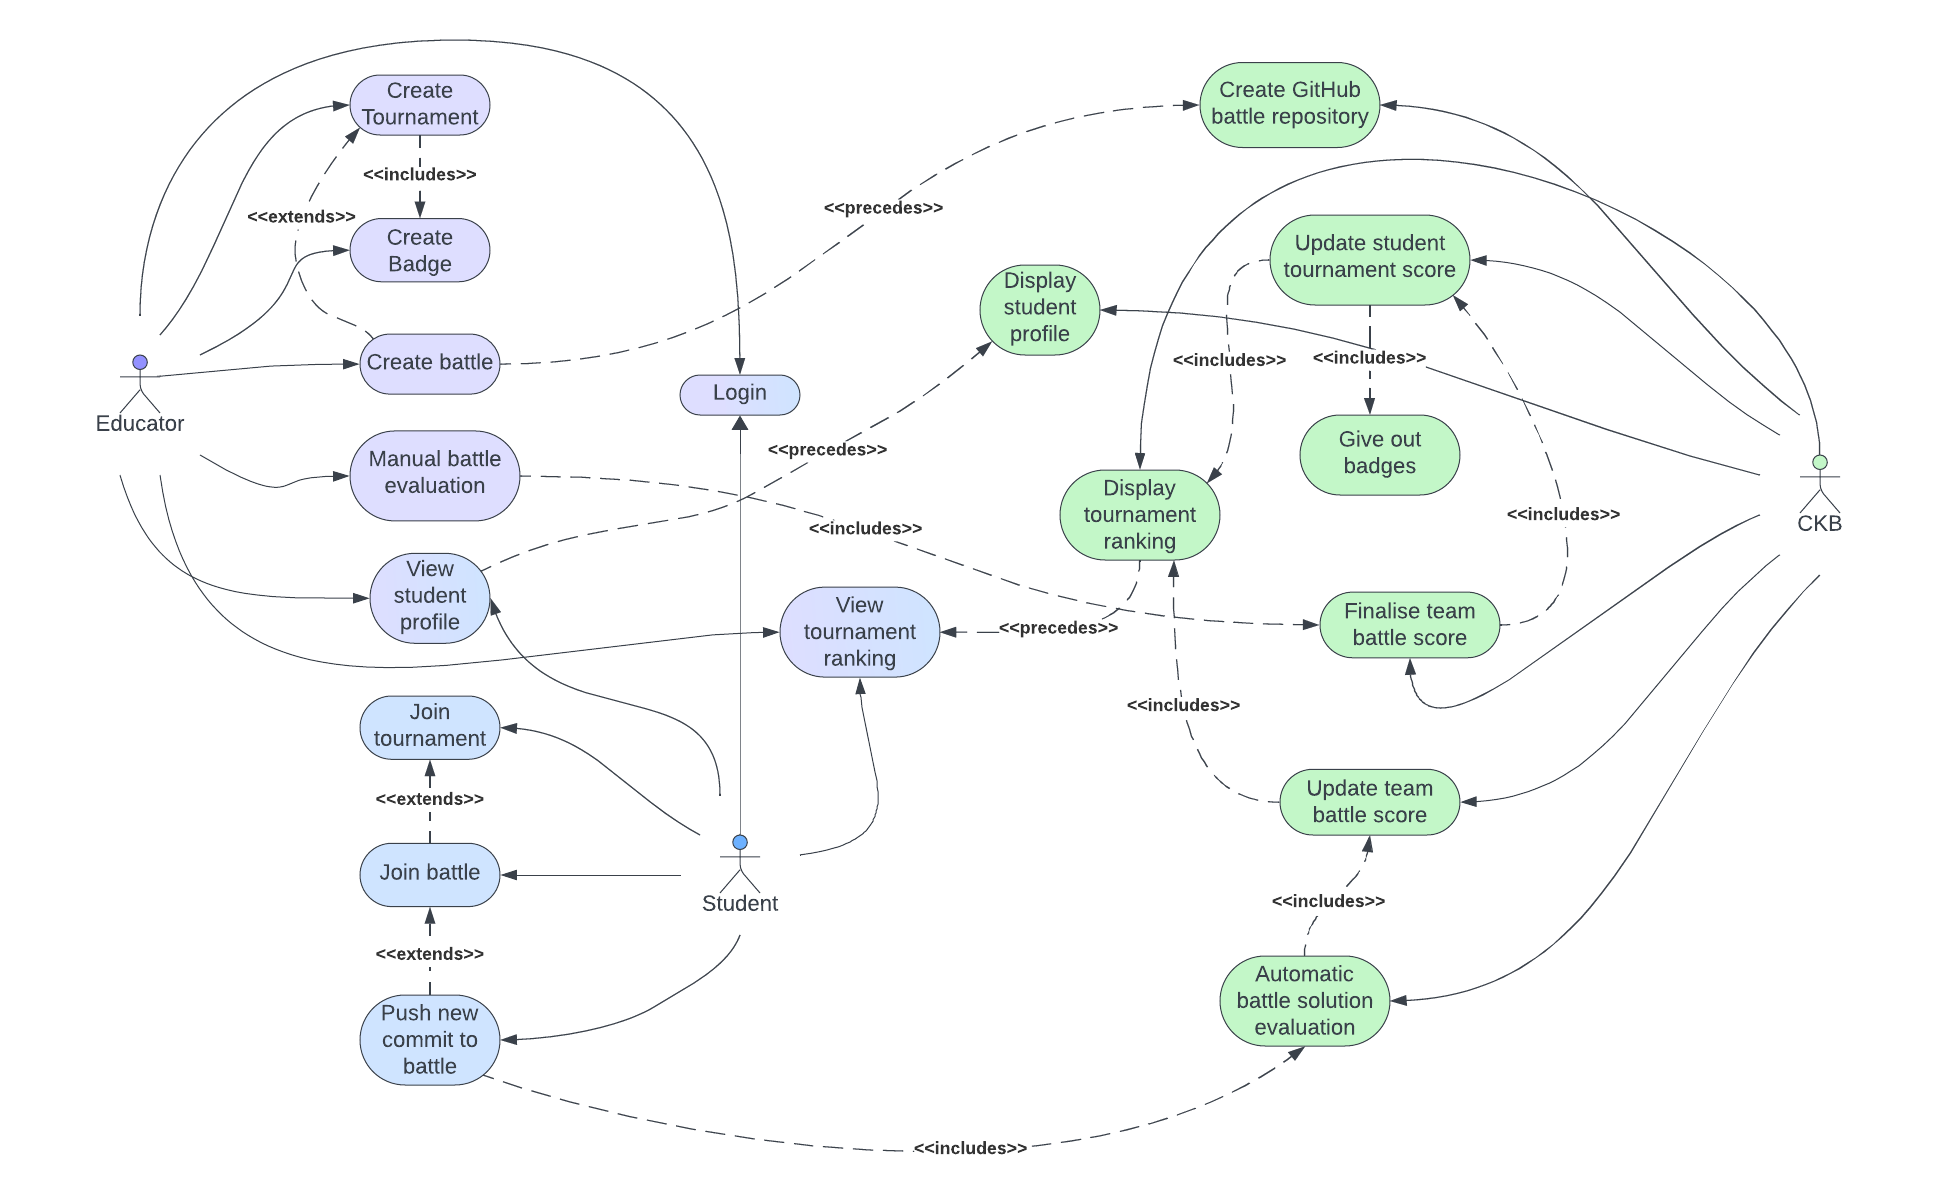
\includegraphics[width=\textwidth]{Graphics/Use case diagram.png}
\caption{Use case diagram.}
\label{fig:use case diagram}
\end{figure}

\clearpage
\newpage





\subsection{Requirements Mapping}
\label{sec:requirements_mapping}

This section maps the functional requirements and domain assumptions to the specific goals of the CodeKataBattle project. This mapping ensures that each goal is achievable through the fulfillment of certain requirements under the given assumptions.

\subsection{Goals to Requirements and Domain Assumptions}


% Goal 1
\begin{longtable}{|p{0.5\textwidth}|p{0.5\textwidth}|}
\hline
\multicolumn{2}{|c|}{\begin{minipage}{0.9\textwidth}
\centering
\vspace{5pt}
\textbf{[G2] Enable Educators to set up test-driven coding challenges including automated feedback online}
\vspace{5pt}
\end{minipage}} \\
\hline
\textbf{Requirements} & \textbf{Domain Assumptions} \\
\hline
R3-R5 Tournament creation with badges & D4 Educators' understanding of version control \\
R8-R13 Battle setup with technical documents and deadlines & D5 Correct automated testing scripts \\
R19 Manual scoring option for educators & R27 Boolean expressions for badge rules \\
\hline
\end{longtable}

% Goal 2
\begin{longtable}{|p{0.5\textwidth}|p{0.5\textwidth}|}
\hline
\multicolumn{2}{|c|}{\begin{minipage}{0.9\textwidth}
\centering
\vspace{5pt}
\textbf{[G2] Enable Educators to set up test-driven coding challenges including automated feedback online}
\vspace{5pt}
\end{minipage}} \\
\hline
\textbf{Requirements} & \textbf{Domain Assumptions} \\
\hline
R3-R5 Tournament creation with badges & D4 Educators' understanding of version control \\
R8-R13 Battle setup with technical documents and deadlines & D5 Correct automated testing scripts \\
R19 Manual scoring option for educators & R27 Boolean expressions for badge rules \\
\hline
\end{longtable}


% Goal 3
\begin{longtable}{|p{0.5\textwidth}|p{0.5\textwidth}|}
\hline
\multicolumn{2}{|c|}{\begin{minipage}{0.9\textwidth}
\centering
\vspace{5pt}
\textbf{[G3] Simulate a Real-world software development scenario through the use of GitHub and GitHub Actions.}
\vspace{5pt}
\end{minipage}} \\
\hline
\textbf{Requirements} & \textbf{Domain Assumptions} \\
\hline
R15 Use of GitHub repositories for code katas & D10 Compatibility with code kata requirements \\
R17 Timeliness evaluation of submissions & D13 Adherence to test-first development approach \\
\hline
\end{longtable}

% Goal 4
\begin{longtable}{|p{0.5\textwidth}|p{0.5\textwidth}|}
\hline
\multicolumn{2}{|c|}{\begin{minipage}{0.9\textwidth}
\centering
\vspace{5pt}
\textbf{[G4] Enable Educators to set up test-driven coding challenges including automated feedback online}
\vspace{5pt}
\end{minipage}} \\
\hline
\textbf{Requirements} & \textbf{Domain Assumptions} \\
\hline
R22 Update of personal tournament scores & D14 Use of scores for constructive feedback \\
R23 Maintenance of visible tournament rank & D15 Fair use of the platform by users \\
R28-R30 Performance visualization tools &  \\
\hline
\end{longtable}

\subsection{Sequence Diagrams}

\begin{figure}[Htbp!]
    \centering
    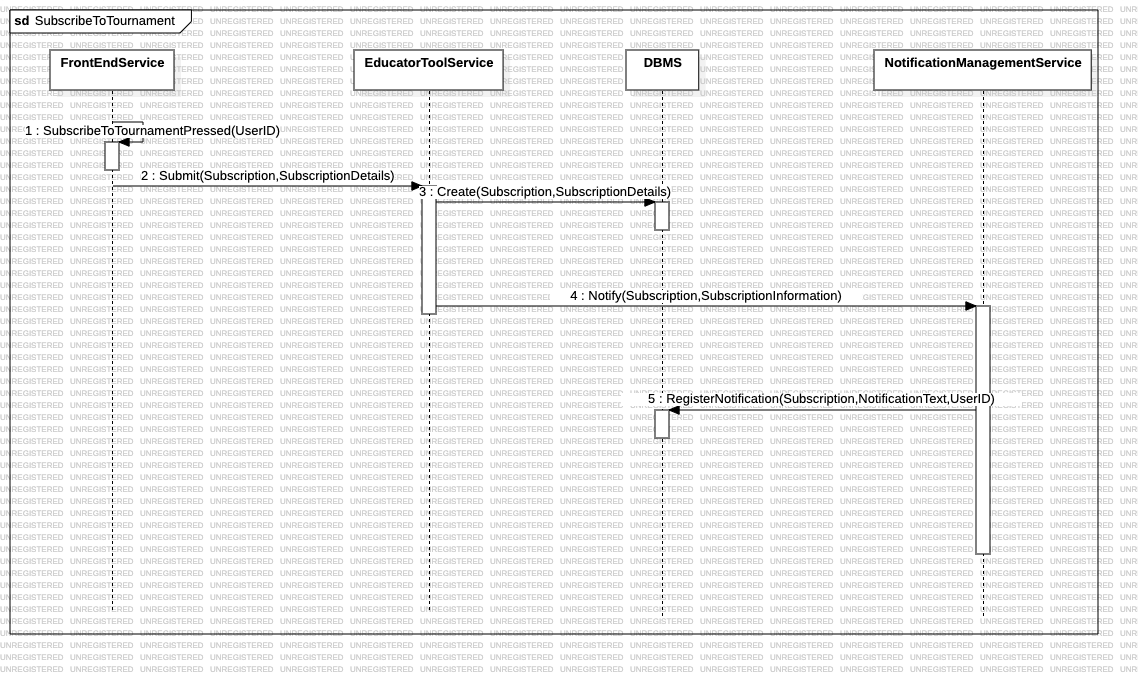
\includegraphics[width=\textwidth]{Graphics/Sequence Diagrams/SubscribeToTournament.png}
    \caption{Sequence Diagram: Subscribe to Tournament}
    \label{fig:Subscribe}
\end{figure}


\begin{figure}[Htbp!]
    \centering
    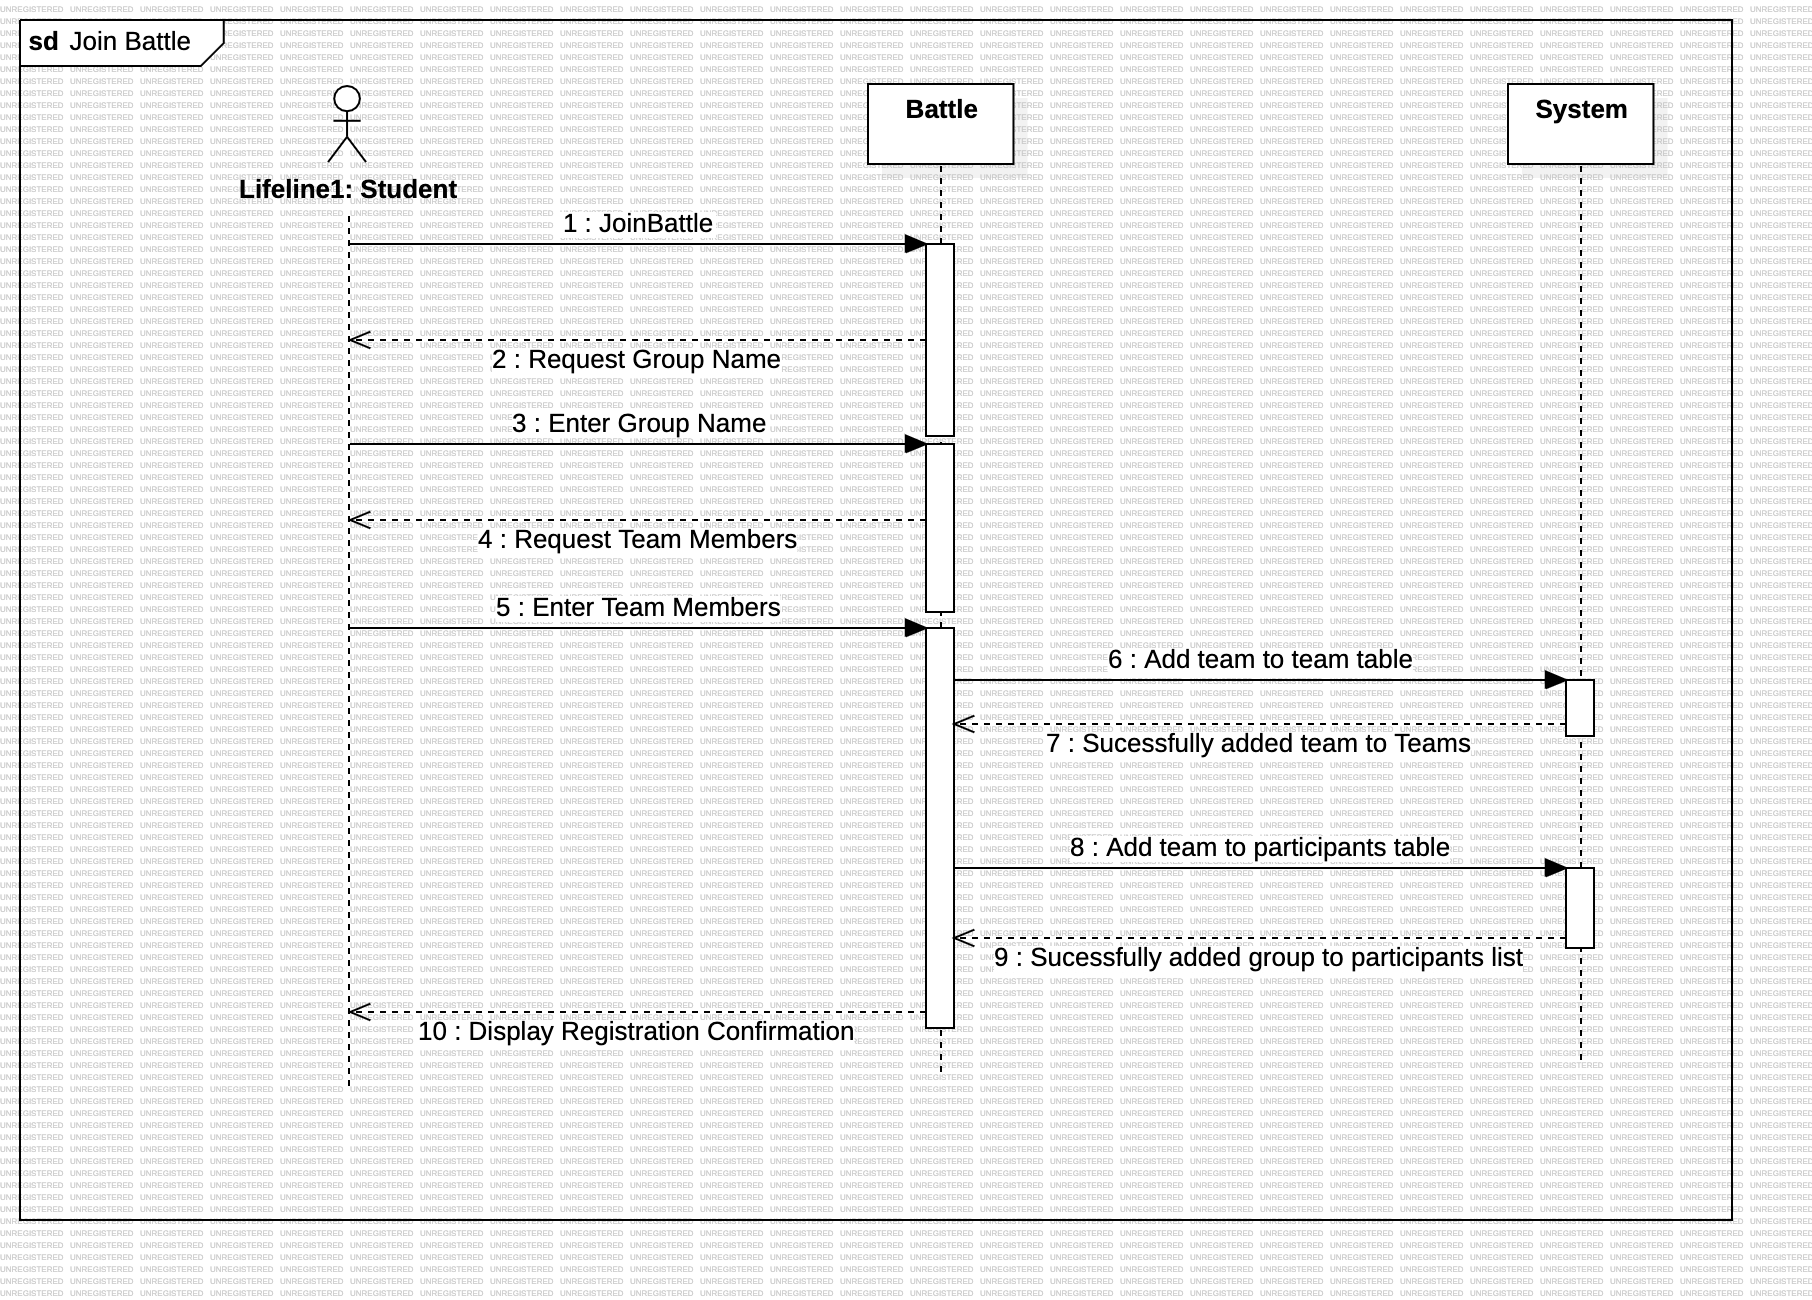
\includegraphics[width=\textwidth]{Graphics/Sequence Diagrams/Join Battle.png}
    \caption{Sequence Diagram: Join Battle}
    \label{fig:Join}
\end{figure}

\newpage

\begin{figure}[Htbp!]
    \centering
    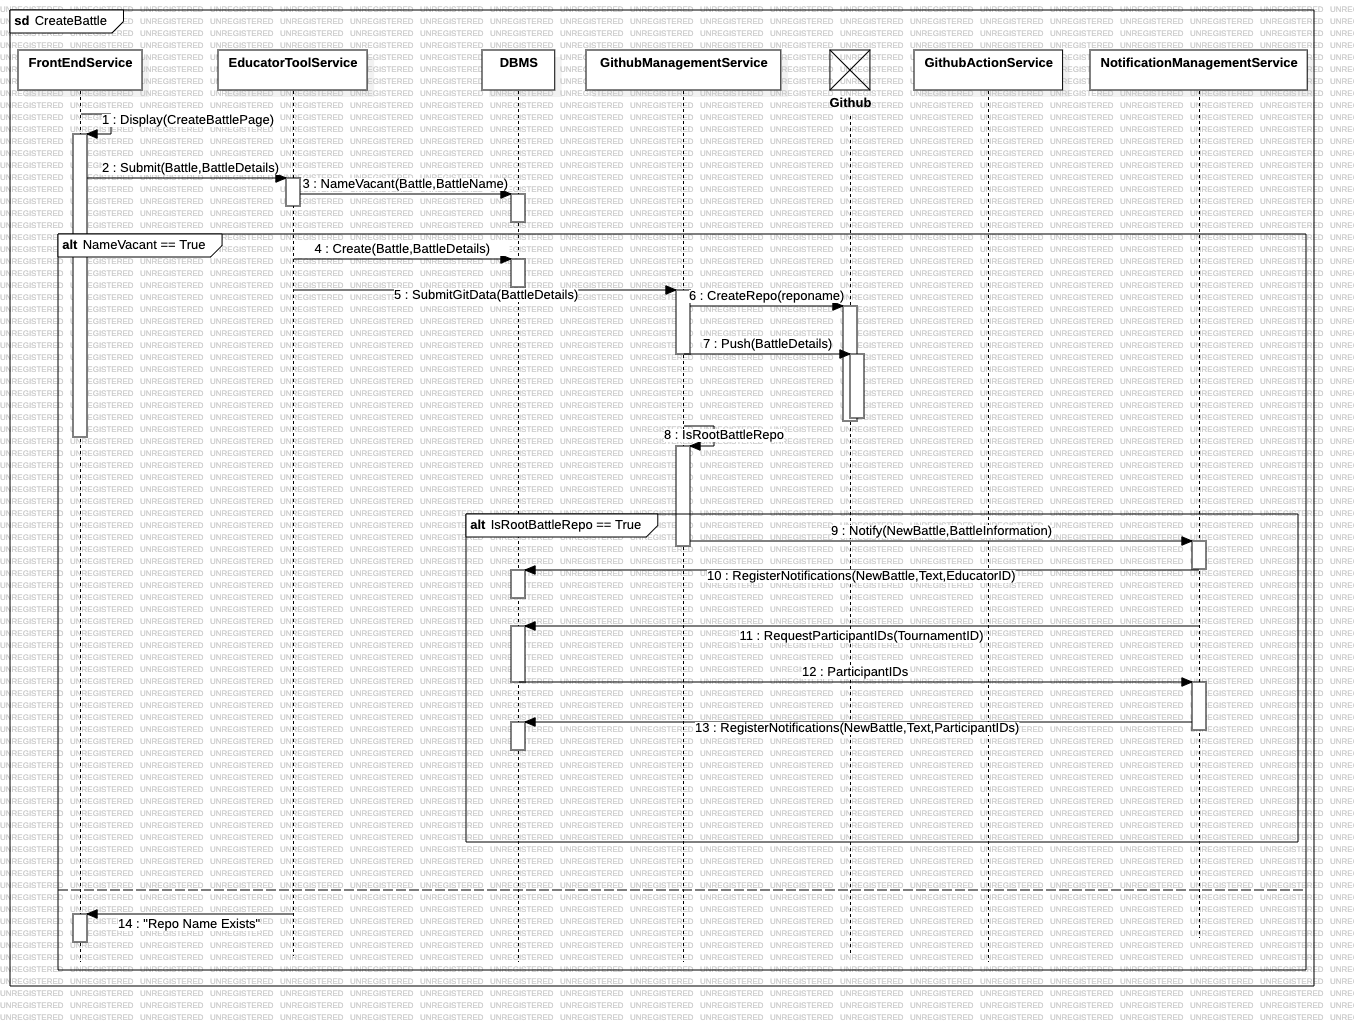
\includegraphics[width=\textwidth]{Graphics/Sequence Diagrams/CreateBattle.png}
    \caption{Sequence Diagram: Create Battle}
    \label{fig:CreateBattle}
\end{figure}



\begin{figure}[Htbp!]
    \centering
    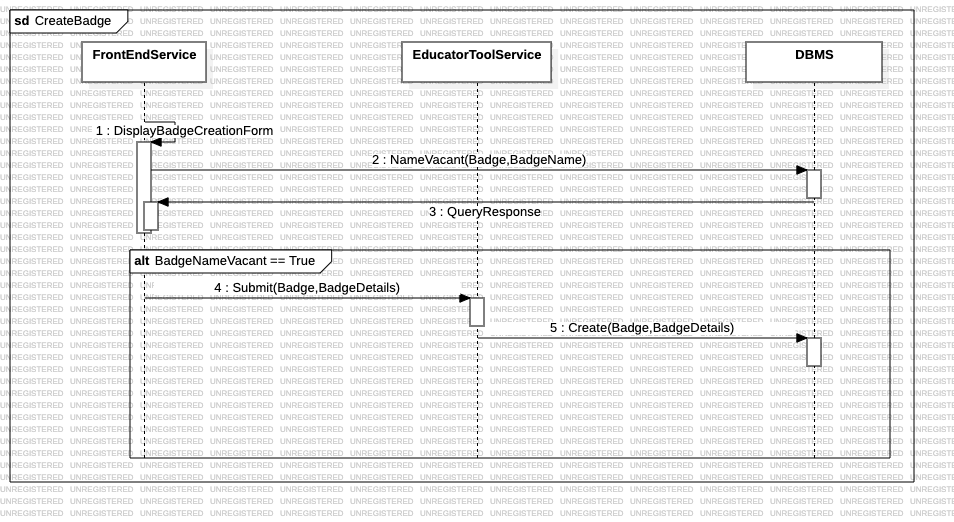
\includegraphics[width=\textwidth]{Graphics/Sequence Diagrams/CreateBadge.png}
    \caption{Sequence Diagram: Create Badge}
    \label{fig:CreateBadge}
\end{figure}
\newpage

\begin{figure}[Htbp!]
    \centering
    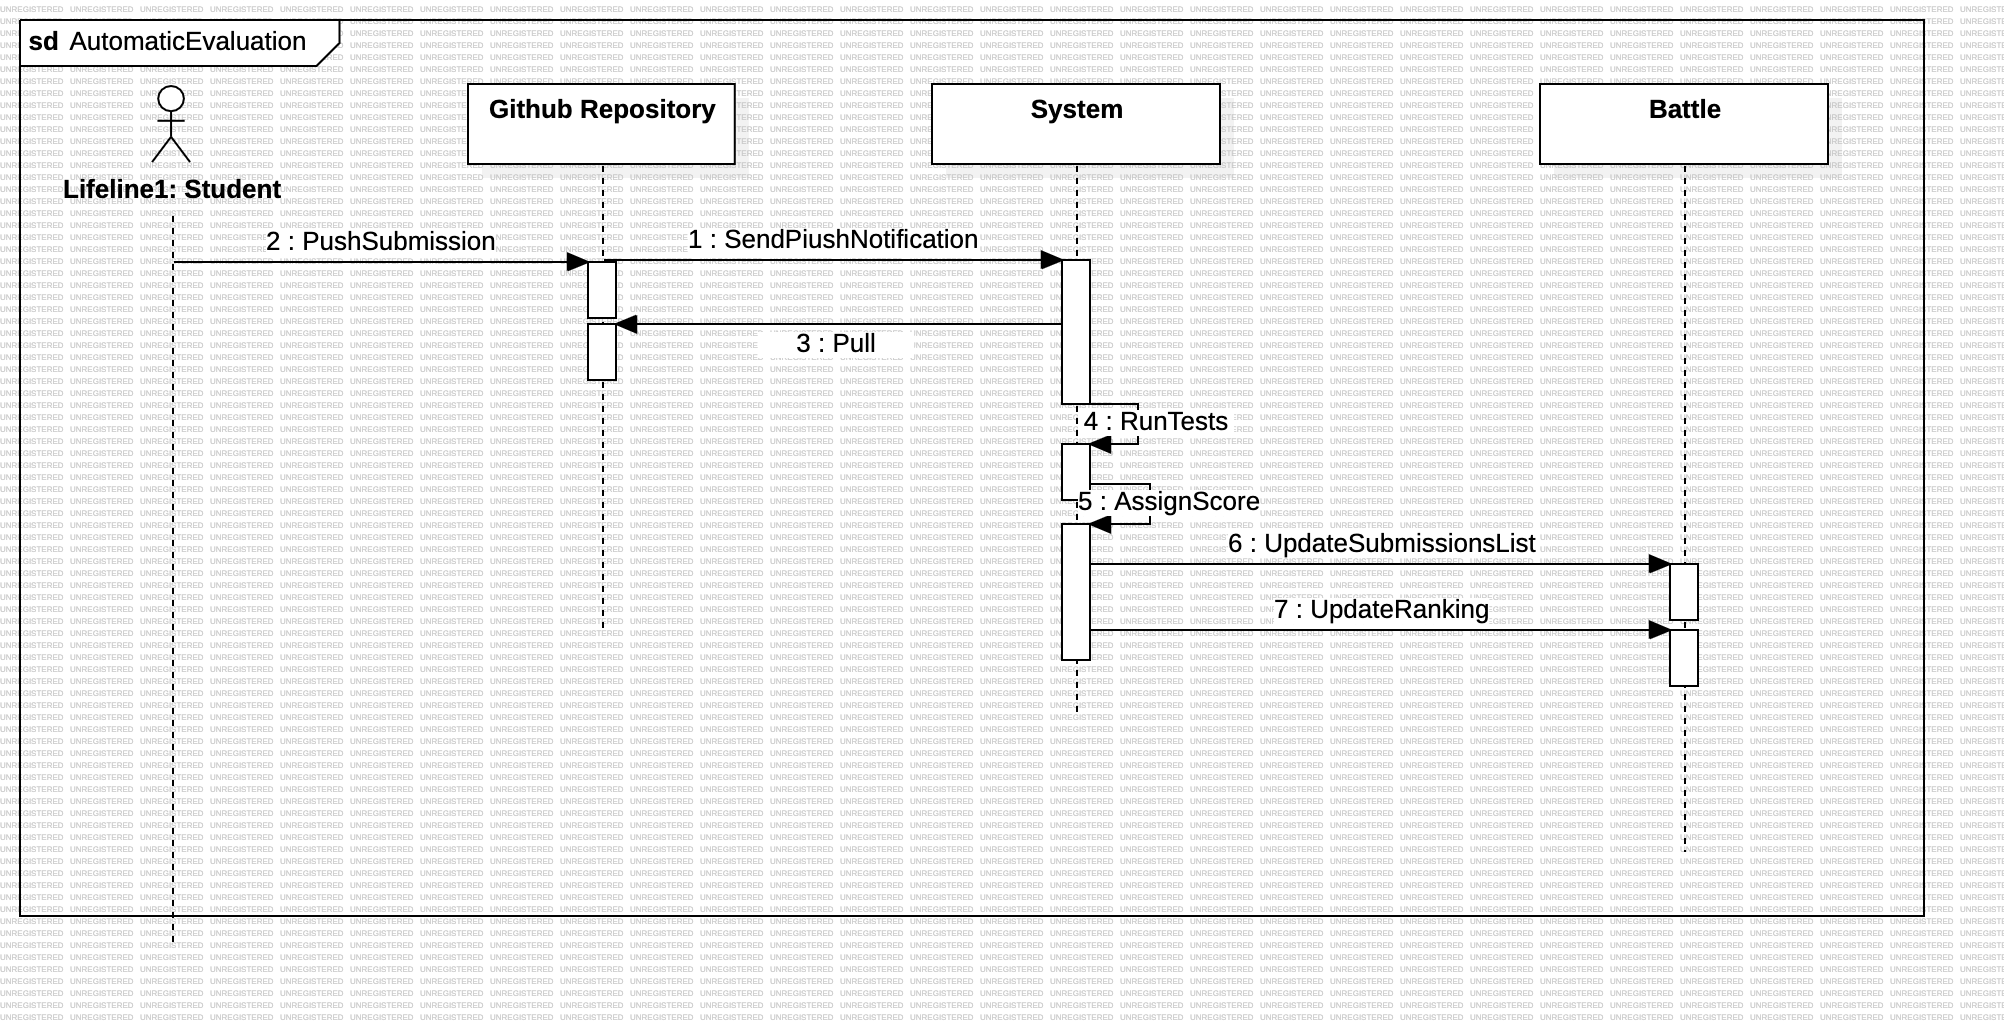
\includegraphics[width=\textwidth]{Graphics/Sequence Diagrams/AutomaticEvaluation.png}
    \caption{Sequence Diagram: Automatic Evaluation}
    \label{fig:AutoEval}
\end{figure}


\begin{figure}[Htbp!]
    \centering
    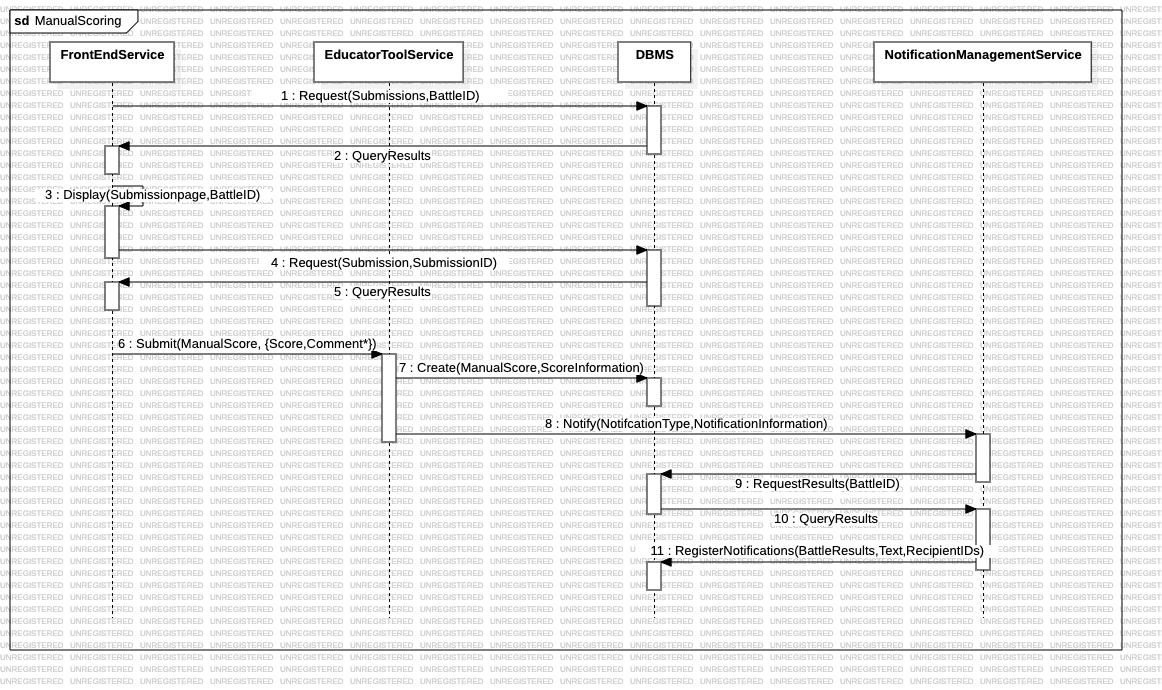
\includegraphics[width=\textwidth]{Graphics/Sequence Diagrams/ManualScoring.png}
    \caption{Sequence Diagram: Manual Evaluation }
    \label{fig:ManEval}
\end{figure}

\newpage
\begin{figure}[Htbp!]
    \centering
    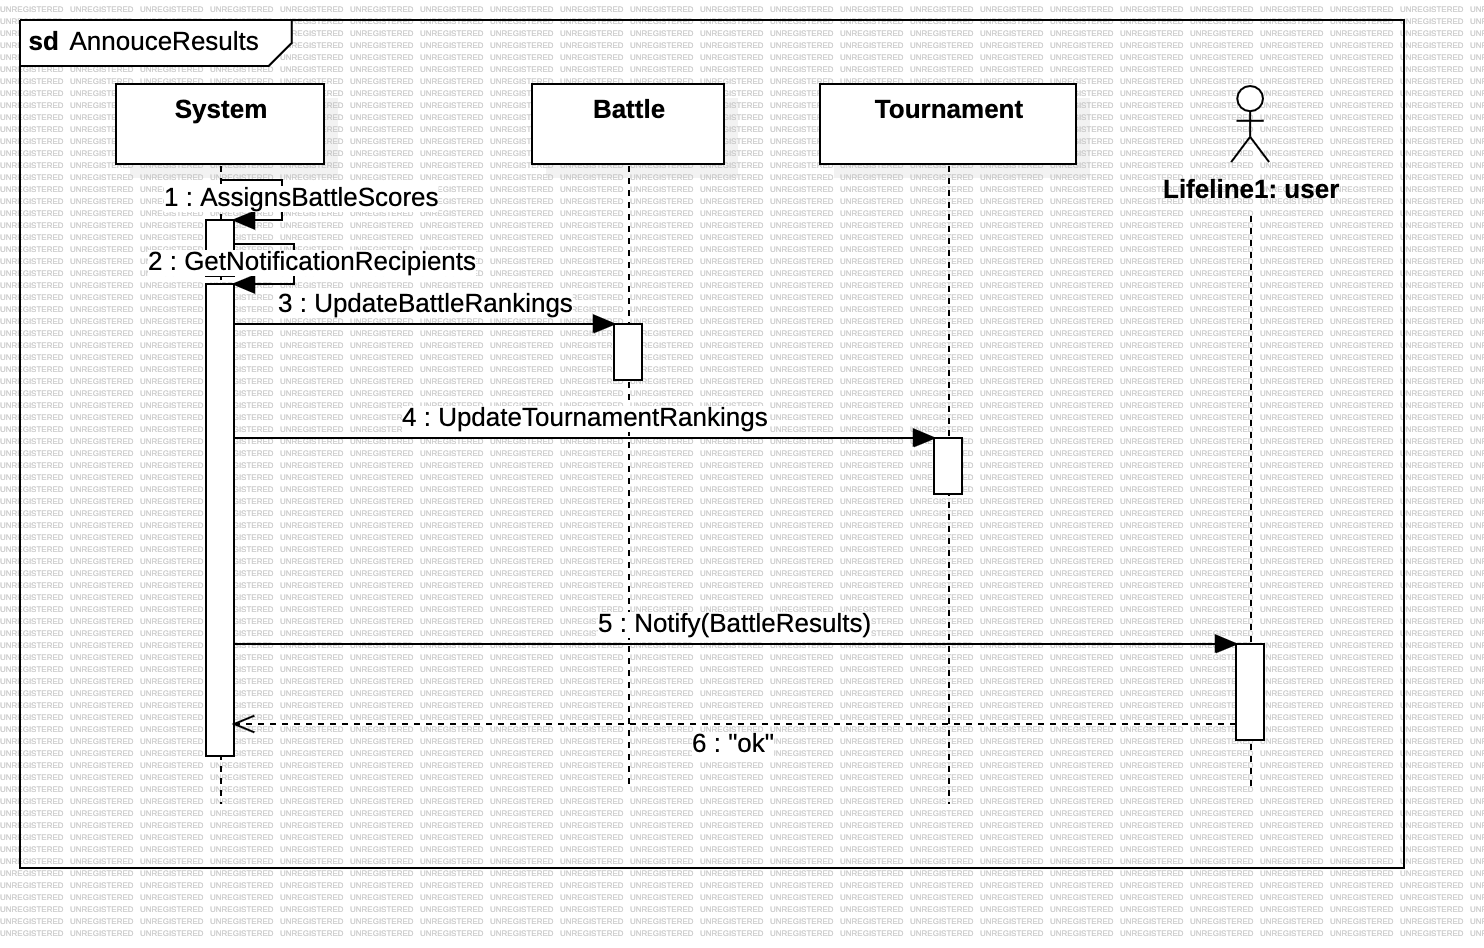
\includegraphics[width=\textwidth]{Graphics/Sequence Diagrams/AnnouceResults.png}
    \caption{Sequence Diagram: Announce Battle Results}
    \label{fig:Announcement}
\end{figure}



\begin{figure}[Htbp!]
    \centering
    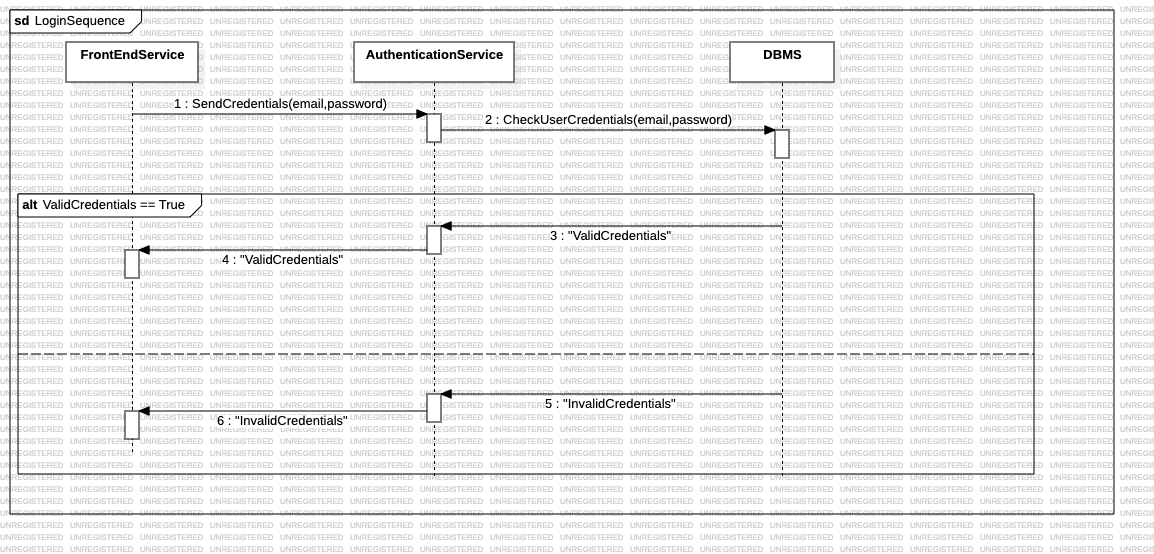
\includegraphics[width=\textwidth]{Graphics/Sequence Diagrams/LoginSequence.png}
    \caption{Sequence Diagram: Log-in Sequence}
    \label{fig:login}
\end{figure}

\newpage
\section{Implementation, Integration \& Test Plan}
This section will specify a plan for implementing the CodeKata Battle system. This includes the specification of system features, the order of their implementation, a strategy to integrate these components into a system, and finally a strategy to test the system as a whole. These tests aim to increase the robustness of the system before, getting into the user's hands. 

\subsection{Implementation Plan}
To ensure implementation is going in the right direction we will be using an iterative development strategy. Here components will be tested as a unit and how they fit into the current iteration of the systems as it is developed. As the CodeKata Battle system consists of few components relative to most systems, we thought a hierarchical approach would be the best fit. Here the components are implemented based on a hierarchical view of the components relations. 

Specifically, we have chosen to employ a top-down approach, as it enables us to tackle integrating some of the more complex components like Github actions. Tackling this problem early in implementation is meant to decrease the likelihood of problems later in the integration process. Going top-down also means tackling the issues of user interfaces and high-level functionalities early on in the development process. Enabling early visualization of progress and feedback from stakeholders. A hierarchal approach in general allows for teams to work in parallel, which is key for avoiding potential bottlenecks.


%\subsubsection{Overview}
%\subsubsection{Iterative Development}
\subsubsection{Technology Stack}

\subsection{Feature Identification}

In this section, we have listed all features comprising the CKB system. This is extracted from the system requirements, and the requirements in the RASD. 

\begin{itemize}
\renewcommand{\labelitemi}{}
    \item \textbf{[F1] User Authentication and Profile Management}
    \begin{itemize}
        \item Basic functionalities for account creation and login.
        %\item Profile overview displaying achievements and participation.
    \end{itemize}

    \item \textbf{[F2] Battle Creation and Management}
    \begin{itemize}
        \item Educators can upload code katas, including descriptions and test cases.
        \item Setting parameters for challenges: group size limits, deadlines, and scoring configurations.
    \end{itemize}

    \item \textbf{[F3] Tournament Creation and Management}
    \begin{itemize}
        \item Creation and configuration of tournaments by educators.
        \item Notification system for new tournaments and student subscriptions.
    \end{itemize}

    \item \textbf{[F4] Student Battle Participation }
    \begin{itemize}
        \item Enrollment and team creation for battles within size limits.
        \item Forking and setting up GitHub repositories for code submissions.
    \end{itemize}

    \item \textbf{[F5] Real-Time Feedback and Scoring}
    \begin{itemize}
        \item Automated evaluation of code based on test cases, timeliness, and code quality.
        \item Optional additional manual scoring parameter by educators.
    \end{itemize}

    \item \textbf{[F6] Tournament and Battle Score Aggregation}
    \begin{itemize}
        \item Automated calculation of individual battle scores.
        \item Compilation of tournament scores from individual battle performances.
    \end{itemize}

    \item \textbf{[F7] Gamification and Badges}
    \begin{itemize}
        \item System for educators to create badges.
        \item Automatic assignment of badges based on rule fulfillment.
    \end{itemize}

    \item \textbf{[F8] Integration with External Services}
    \begin{itemize}
        \item GitHub integration for code repository management and automated testing.
    \end{itemize}

    \item \textbf{[F9] User Notification System}
    \begin{itemize}
        \item Automated notifications for updates, deadlines, and results.
        %\item Customizable notification preferences for users.
    \end{itemize}

    \item \textbf{[F10] Profile Visualization of Achievements}
    \begin{itemize}
        \item Feature to display collected badges on student profiles.
        \item Visibility of ongoing tournament details and individual rankings.
    \end{itemize}
\end{itemize}




\subsection{Integration Plan}
\subsubsection{Component Integration}

Here is a prioritized list of orders in which we intend to implement components following the top-down approach stated in the implementation strategy. Unit testing will require the creation of test stubs to accurately simulate components functionality. Unit testing is intended to be done after each component is finished, whereafter an integration test is performed to ensure components interaction perform as expected. 

\begin{itemize}

    \renewcommand{\labelitemi}{}

    \item \textbf{[C1] Front-end Service}
    \begin{itemize}
        \item The Front-end Service is the primary user interface, and for this reason, it is important for initial user feedback and specifying the requirements for backend services.
    \end{itemize}


    \item \textbf{[C2] Data Persistence Service (DBMS)}
    \begin{itemize}
        \item As the backbone of the system, storing all persistent data, the database is integrated last to support all other services, once there is a clear understanding of the data requirements.
    \end{itemize}

    \item \textbf{[C3] GitHub Management Service}
    \begin{itemize}
        \item Manages the creation and updates of GitHub repositories, integral to the platform's code submission and review process. Its integration follows the Notification Management Service to ensure that repositories are managed alongside user notifications.
    \end{itemize}

    \item \textbf{[C4] Authentication Service}
    \begin{itemize}
        \item Authentication Service is a core functionality to the very first user interface users interact with, and vital to security and user management. This service must be integrated early to facilitate secure access and testing of subsequent components.
    \end{itemize}

    \item \textbf{[C5] Scoring Service}
    \begin{itemize}
        \item Integral to the competitive aspect of the platform, the Scoring Service is developed after core functionalities to allow for contextualized scoring within tournaments.
    \end{itemize}

    \item \textbf{[C6] GitHub Actions}
    \begin{itemize}
        \item GitHub Actions underpin the automated testing functionality and are critical to operations. They are integrated after the essential user and battle management services are established.
    \end{itemize}
    
    \item \textbf{[C7] User Profile Service}
    \begin{itemize}
        \item Closely tied to user interaction, this service is integral for personalization and displaying user-specific data, and therefore prioritized early in the process.
    \end{itemize}
    
    \item \textbf{[C8] Educator Tools Service}
    \begin{itemize}
        \item This service enables educators to create content, a core functionality of the platform. Its integration is prioritized to test the creation and management of challenges.
    \end{itemize}

    %\item \textbf{[C5] Tournament Management Service}
    %\begin{itemize}
       % \item This service manages the logical grouping of battles into tournaments and is integrated after the Educator Tools Service to facilitate the management of these entities.
    %\end{itemize}
    
    \item \textbf{[C9] Notification Service}
    \begin{itemize}
        \item Notifications keep users engaged and informed. This service is prioritized following user authentication to ensure effective communication within the platform.
    \end{itemize}

    \item \textbf{[C10] Badge Management Service}
    \begin{itemize}
        \item As part of the gamification strategy, this service is integrated after the Notification Service to utilize the infrastructure for user communication.
    \end{itemize}
\end{itemize}

%\subsubsection{API Integration}
%
%\subsection{Test Plan}
%\subsubsection{Unit Testing}
%\subsubsection{Integration Testing}
\subsection{System Testing}
After having integrated all components together, we will have a system that can be tested as a whole. System testing intends to ensure the system as a whole meets all functional and non-functional requirements. To do this the system must undergo several different types of testing phases as laid out in the following section.

\begin{itemize}
    \item[] \textbf{Functional Testing}: This phase checks if the system complies with all the requirements specified in the Requirement Analysis and Specification Document (RASD). This will be done by trying to execute the use case scenarios and see if the system complies with the intended outcomes.

    \item[] \textbf{Performance Testing}: The system will be evaluated to identify any potential performance bottlenecks, such as inefficient elements that may impact response times or resource utilization. To check this testing the system under the expected workload will be done. 
    
    \item[] \textbf{Usability Testing}: To ensure the system is both intuitive and easy-to-use, we'll have a person outside the development team evaluate the system. 
    
    \item[] \textbf{Load Testing}: The system will be tested under increasing loads to discover bugs that may not surface under normal operation, such as memory leaks or buffer overflows. It will also help determine the system's maximum operating capacity over extended periods.
    
    \item[] \textbf{Stress Testing}: This testing ensures the system can handle and recover from adverse conditions. It involves overwhelming the system's resources or depriving it of them to see how it behaves under extreme stress.

\end{itemize}



%\begin{itemize}
%    \item Functional Testing
%    \item Performance Testing
%    \item Usability Testing
%    \item Interoperability Testing
%    \item Load Testing?
%    \item Recovery Testing
%\end{itemize}
\clearpage
\newpage
\section{Efforts Spent}
\label{sec:effort}
The tables below indicate how much time each participant has spent on each of the sections in the report. 

\subsection{Karl Kieler}
\begin{table}[h]
\centering
\begin{tabular}{|c|c|}
\hline
Section & Time Spent (Hours) \\ \hline
Introduction & 2 \\ \hline
Overall Description & 11 \\ \hline
Specific Requirements & 16 \\ \hline
Formal Analysis & 12 \\ \hline
\end{tabular}
\end{table}


\subsection{Leonie Dragun}
\begin{table}[h]
\centering
\begin{tabular}{|c|c|}
\hline
Section & Time Spent (Hours) \\ \hline
Introduction & 4 \\ \hline
Overall Description & 12 \\ \hline
Specific Requirements & 16 \\ \hline
Formal Analysis & 12\\ \hline
\end{tabular}
\end{table}


\subsection{Aske Schytt Meineche}
\begin{table}[h]
\centering
\begin{tabular}{|c|c|}
\hline
Section & Time Spent (Hours) \\ \hline
Introduction & 4 \\ \hline
Overall Description & 9 \\ \hline
Specific Requirements & 19 \\ \hline
Formal Analysis & 12 \\ \hline
\end{tabular}
\end{table}

\newpage
\section{References}
\label{sec:ref}

\begin{enumerate}
    \item Diagrams made with: StarUML and Microsoft PowerPoint
    \item Mockups made with Microsoft PowerPoint
\end{enumerate}




%\bibliography{refs}

\end{document}
